\documentclass[compsoc]{IEEEtran}
\IEEEoverridecommandlockouts

% \documentclass[letterpaper,twocolumn,10pt]{article}
%\usepackage{usenix-2020-09}
\usepackage{graphicx}
\usepackage{subfig}
%Removing the geometry package used for Tighter Format
%\usepackage{geometry}
%\usepackage{times}
\usepackage{textcomp}
\usepackage{multirow}
\usepackage{framed}
\usepackage{amsmath}
\usepackage{listings}
\usepackage{comment}
\usepackage{booktabs}

\usepackage[noend]{algpseudocode}
\usepackage[nothing]{algorithm}

% \usepackage[hyphens]{url}
\PassOptionsToPackage{hyphens}{url}
\usepackage{hyperref}
%\usepackage{hyperref}
\usepackage{enumitem}
\usepackage{amssymb}

\usepackage[colorinlistoftodos,prependcaption,textsize=footnotesize]{todonotes}
\newcommand{\todocristina}[1]{\todo[inline, color=blue!60]{\textbf{Cristina}: #1}}
\newcommand{\todoprateek}[1]{\todo[inline, color=yellow!60]{\textbf{Prateek}: #1}}
\newcommand{\todojose}[1]{\todo[inline, color=red!60]{\textbf{José}: #1}}
\newcommand{\todoall}[1]{\todo[inline, color=green!60]{\textbf{Comment}: #1}}


%Used only for breaking hypenated URLs
\usepackage{etoolbox}
\gappto{\UrlBreaks}{\UrlOrds}
%

\hypersetup{breaklinks=true}

\urlstyle{same}

\begin{document}
\date{}

\title{Priority- and Locality-aware Load Balancing For Serverless Clusters}
% \title{Serverless Cluster Management using Locality and Stale-load aware Policies}
% \title{Combining Locality and Stale-load awareness for Serverless Load Balancing}

% ABOUT AUTHOR ORDER: I am using the one we had discussed months ago. We can change it to, for example, the alternate author order shown below.
%Alternate author order based 100% on contribution: Prateek, Cristina, Alexandre, José, Robinson
% \author{Alexander Fuerst,~\IEEEmembership{Student Member,~IEEE,}
%         Jos\'{e} Viteri,
%         Robinson Flores,
%         Prateek Sharnma,~\IEEEmembership{Member,~IEEE,}
%         Cristina L. Abad,~\IEEEmembership{Senior Member,~IEEE,}%% <-this % stops a space
% \IEEEcompsocitemizethanks{\IEEEcompsocthanksitem A. Fuerst and P. Sharma are with Indiana University, Bloomington-USA\protect\\
% % note need leading \protect in front of \\ to get a newline within \thanks as
% % \\ is fragile and will error, could use \hfil\break instead.
% E-mail: \{alfuerst,prateeks\}@iu.edu
% \IEEEcompsocthanksitem J. Viteri, R. Flores and C. Abad are with Escuela Superior Politecnica del Litoral, Guayaquil-Ecuador.\protect\\
% E-mail: \{javiteri,rjflores,cabadr\}@espol.edu.ec}% <-this % stops an unwanted space
% %\thanks{Manuscript received April 19, 2005; revised August 26, 2015.}
% }
\author{Alexander Fuerst,
        Prateek Sharnma,
        Cristina L. Abad}
      
%\IEEEcompsocitemizethanks{\IEEEcompsocthanksitem A. Fuerst and P. Sharma are with Indiana University, Bloomington-USA\protect\\
% note need leading \protect in front of \\ to get a newline within \thanks as
% \\ is fragile and will error, could use \hfil\break instead.

%      E-mail: \{alfuerst,prateeks\}@iu.edu
%\IEEEcompsocthanksitem C. Abad is with Escuela Superior Politecnica del %Litoral (ESPOL), Guayaquil-Ecuador.\protect\\
%E-mail: cabadr@espol.edu.ec}% <-this % stops an unwanted space
%\thanks{Manuscript received April 19, 2005; revised August 26, 2015.}
%}


\maketitle

\begin{abstract}
  
Functions as a Service (also called serverless computing) promises to revolutionize how applications use cloud resources. 
However, functions suffer from cold-start problems due to the overhead of initializing their code and data dependencies before they can start executing. 
Keeping functions alive and warm after they have finished execution can alleviate the cold-start overhead. 
Keep-alive policies must keep functions alive based on their resource and usage characteristics, which is challenging due to the diversity in FaaS workloads. 


Our insight is that keep-alive is analogous to caching.
Our caching-inspired Greedy-Dual keep-alive policy can be effective in reducing the cold-start overhead by more than $3\times$ compared to current approaches. 
Caching concepts such as reuse distances and hit-ratio curves can also be used for auto-scaled server resource provisioning, which can reduce the resource requirement of FaaS providers by $30\%$ for real-world dynamic workloads. 
We implement caching-based keep-alive and resource provisioning policies in our FaasCache system, which is based on OpenWhisk. 
We hope that our caching analogy opens the door to more principled and optimized keep-alive and resource provisioning techniques for future FaaS workloads and platforms. 



%%% Local Variables:
%%% mode: latex
%%% TeX-master: "paper"
%%% End:

\end{abstract}



\section{Introduction}

Function as a Service (also called FaaS or serverless computing) is one of the fastest growing abstractions in cloud computing today with usage increasing by 2x in the past two years alone~\cite{wen2023rise}.
% Users create self-contained \textit{functions} whose lifecycle is orchestrated by the FaaS provider.  
Users are enticed by its dynamic scaling, low cost, and ease of management, as the lifecycle of self-contained \textit{functions} is orchestrated by the FaaS provider.
% Cloud providers benefit because functions use ephemeral resources unlike traditional virtual machines (VMs) and the provider has find-grained control over scheduling and placement.
Cloud providers leverage the ephemeral nature of functions into fine-grained control over scheduling, placement, and resource allocation.

% 1)
Current FaaS applications are limited by the capabilities exposed by providers, mostly consisting of short-running functions~\cite{shahrad2020serverless} using limited compute.
% Functions are given limited CPU resources and have no way efficient of coordinating with one another, precluding classic parallel computing.
Providers have not exposed GPUs or other parallel processing paradigms to their serverless platforms, a need for which is growing as users migrate new, intensive, workflows to cloud FaaS.
These applications see a \emph{minimum} 2.5x throughput improvement when accelerated, strong encouragement to enable such devices in serverless platforms.

% 2-3)
Accomplishing this transition requires the control plane to address several resource management problems.
Achieving high device utilization and low latency require device multiplexing~\cite{pemberton2022kernel, ng2023paella, fingler2022dgsf, gu2023fast}, but unmodified functions preclude such sharing of GPU resources.
% To make matters more complicated, GPU resources are managed by an esoteric device driver that isn't controllable by the OS.
Once a function is given access to the GPU, it can allocate the entire memory range or hog compute in a run-to-completion model.
% Idle periods mean allocated resources on the GPU are blocked off, other functions being unable to use them for their executions.
% Removing containers to release held resources results in heavy churn and increased latency from the repeated container initialization.
Swapping functions requires starting a new container, costing several seconds on the critical path, making the well-known \quotes{cold start} problem of FaaS an even larger latency bottleneck.
% We avoid cold starts by being the first to enable GPU keep-alive~\cite{faascache-asplos21} policies via GPU resource multiplexing.
Avoiding cold starts (i.e. a warm start) to get viable performance requires enabling GPU keep-alive~\cite{faascache-asplos21} policies via GPU resource multiplexing.

\begin{comment}
Machines used to host FaaS systems are expected to serve thousands of unique functions with low latency.
This is accomplished by running user function code inside a container (or VM), then keeping the container in memory but idle for future uses. 
A na\"ive adaption of this to the GPU problem would assign an entire GPU to each container for its lifetime.
Unfortunately an idle container then wastes GPU resources, and the limited number of GPUs per server leads to churn when we need to create a new container for another function.
% but this causes low utilization and high turnover when going to run a new function.
Virtualization for these devices exists, provisioning fixed slices of GPU resources to containers that they then have exclusive access to.
% This also results in low utilization, as nothing else can use that section when it is idle, and also limits the resources available to give to any one function that might take advantage of them.
While allowing more containers to exist concurrently, this solution does not address idleness and introduces a new limitation by reducing the maximum allocation any single function is allowed to make.
\end{comment}
  
% 4-6)
Multiplexed resources are not a performance panacea: the platform must now contend with function fairness and locality.
% The FaaS control plane must also guarantee that all functions will run in a timely and fair manner.
% GPUs must also be shared temporally 
Optimal performance is achieved by running one function repeatedly, as its data dependencies will be available on-device.
Yet a popular function can easily starve others of device time and violate fairness guarantees if not eventually blocked.
% Temporal GPU sharing between the highly heterogeneous serverless workloads must be balanced with execution \quotes{locality}.
New queuing policies tailored to the unique scenario of GPU-serverless computing must be designed to ensure fairness while maintaining high throughput.
% Warm hits, i.e. executing using an already existing container, have up to 100x lower latency compared to their cold counterparts.
% Such execution \quotes{locality} can only come 
% want warm starts.
% locality good -> 'batching'.
% but need spatial/temporal multiplexing as well.

% 7
Previous research work into enabling GPU acceleration in FaaS has focused on ML inference~\cite{pemberton2022kernel, ng2023paella, fingler2022dgsf, gu2023fast}; understandable given its popularity.
These approaches have abandoned the black-box nature of FaaS in favor of extremely fine-grained control of GPU usage and scheduling.
Supporting functions of all types is critical, as more use cases like scientific computing~\cite{kumanov2018serverless,hung2019rapid}, video encoding~\cite{ao2018sprocket, zhang2019video}, and optimization problems~\cite{aytekin2019harnessing,werner2018serverless,shankar2020serverless}, migrate to the platform.
% Our work uniquely enables all these to run natively with minimal overhead.
% Custom solutions have been proposed~\cite{}, but rely on targeted workloads or bespoke platforms, a general-purpose approach is needed.

% 7)
Given these known problems, in this work we seek to answer several research questions:
\begin{enumerate}[leftmargin=*]
  % \item Can we provide GPU acceleration to black-box, unmodified, serverless functions?
  % \item How can GPU support be integrated into high-performance FaaS control planes?
  \item Can we provide GPU acceleration to black-box, unmodified, serverless functions?
  \item Can we multiplex GPU resources between functions in a low overhead manner?
  \item How do we balance locality, fairness, and performance in the face of heterogeneous functions?
  % \item Is this possible without the cost of full virtualization?
\end{enumerate}
% \todo{Better RQs to frame novelty}

In this work, we propose and designed a series of techniques and policies that resolve all of these issues.
They enable black-box serverless functions to utilize GPUs for acceleration while concurrently sharing its resources.
We built our system on top of the \sysname~platform~\cite{fuerst2023iluvatar}, utilizing Nvidia's integration with Docker~\cite{docker-main}. %, but is generic to any accelerator or isolation system.
Importantly, they don't rely on specific hardware or software versioning support, and work on heterogeneous hardware regardless of age or capability. 

% \mhead{RQ1}
Starting from the lowest level component, we interpose an intercept shim between function code and the GPU driver.
Using this, we capture all memory allocation calls and transform them into Unified Virtual Memory (UVM)~\cite{nvidia-uvm} calls.
UVM memory allows applications to allocate beyond the device limits, letting the driver use host memory as swap space, migrating memory on demand. 
Once all allocations are converted to UVM memory, we use the shim to move memory between host and device under direction from the control plane.

% \mhead{RQ2}
Controlling memory positioning allows us to both oversubscribe device memory and keep containers warm while other functions execute on the GPU.
To enable multiple functions to run concurrently, a new queuing policy is required that better matches the new device's capabilities and workload characteristics.
We accomplish this with a modified implementation of a Mutli-Queue Fair Queue (MQFQ)~\cite{hedayati2019multi}, which prevents starvation, scales invocations across multiple GPUs, and minimizes execution overhead.
To prevent contention interference, we monitor device utilization using NVML~\cite{nvml} and track memory usage to throttle invocations.

With these controls we improve function latency by orders of magnitude over previous solutions and expand the pool of serverless applications.
In short, this work proposes the following enhancements to serverless computing:
\begin{enumerate}[leftmargin=*]
  \item We create a custom driver that intercepts function allocation calls to multiplex device memory.
  \item With no limit on device memory, we can keep idle containers resident, creating the first warm pool of GPU containers.
  \item Our memory management techniques allow us to reduce device pressure from idle functions, mitigating overcommitment overhead.
  \item We design a queuing policy that enables concurrent execution while ensuring fairness under heterogeneous workloads.
  % \item W
  % \item Benchmark suite of GPU-enabled serverless functions, including many non-machine learning applications.
\end{enumerate}

This paper is ordered as follows.
Section~\ref{sec:bg} covers background of serverless work and GPU virtualization.
Our motivation behind work is explained in detail in Section~\ref{sec:motiv}.
Section~\ref{sec:design} details our design of queuing, memory control, and resource management.
We examine the implementation of these pieces in Section~\ref{sec:impl}.
Lastly, Section~\ref{sec:eval} shows the effectiveness of our systems with a thorough experiment suite.


%Background and related work. 
%background on serverless platforms and keep-alive

% This is an introductory paragraph talking about serverless computing and some context. Seems repetitive wrt introduction? 
Serverless computing is now being provided by all large public cloud providers: Amazon Lambda, Google Functions, and Azure Functions are becoming an increasingly popular way to deploy applications on the cloud.  
Functions as a Service (FaaS) can also be realized on private clouds and dedicated clusters through the use of frameworks such as OpenWhisk~\cite{openwhisk}, OpenFaas~\cite{openfaas}, OpenLambda~\cite{hendrickson2016serverless}, etc. 
%
In this new cloud paradigm, users provide functions in languages such as Python, Javascript, Go, and others. 
%
The functions are executed by the FaaS platform, greatly simplifying resource management for the application. 



% Need to explain how it all works. But first provide some context for why this is important.


%In order to provide FaaS, the way it is implemented by platforms, results in certain performance challenges.
However, the execution of FaaS functions entails performance overheads that we must be cognizant of. 
%
%FaaS functions cannot assume that state will persist across invocations, and functions need to be self contained in terms of their dependencies. 
%
FaaS functions cannot assume that state will persist across invocations, and function definitions must first import and load all code and data dependencies on each execution. 
%
Each functions is run inside a containers such as Docker~\cite{docker-main}, or a lightweight VM such as Firecracker~\cite{firecracker-nsdi20}. 
By encapsulating all of the function state and any side-effects, the virtual execution environment provides isolation among multiple functions, and also allows for concurrent invocations of the same function. 
%
Due to the overhead of starting a new virtual execution environment (i.e., container or VM), and initializing the function by importing libraries and other data dependencies, function execution thus incurs a significant ``cold start'' penalty. 
%
Thus, FaaS can result in significant performance (i.e., total function execution latency) overheads compared to conventional models of execution where applications can reuse state and do not face the high initialization overheads. 


Two main techniques are used to alleviate the cold start penalty. 
Once a container for a function is created and the function finishes execution, the container can be kept alive instead of immediately terminating it. 
Subsequent invocations of the function can then \emph{reuse} the already running container.
This \emph{keep-alive} mechanism can alleviate the cold start overhead due to container launching (which can be $\sim 100$ ms). %Might be confusing, keep-alive also helps in other initialization. 
The second technique for reducing the cold start overhead is to explicitly initialize functions before running them, and resolving most of the function's code and data dependencies during the initialization phase. 

An example of function initialization is shown in Figure~\ref{fig:lambda-example}, which shows a pseudo-code snippet of a function that performs machine learning inference on its input. 
For ML inference, the function downloads an ML model and initializes the TensorFlow ML framework (lines  5 and 6). 
If the function's container is kept alive, then invocations of the function do not need to run the expensive initialization code (lines 2--6). 
Thus, the execution latency of functions can be minimized with a combination of careful function  initialization and keeping the containers alive. 


% \footnotesize
\begin{figure}
\begin{lstlisting}[language=Python, numbers=left, frame=single, basicstyle=\sffamily, columns=fullflexible]
#Initialization code 
import numpy as np 
import tensorflow as tf
  
m = download_model('http://model_serve/img_classify.pb')
session = create_tensorflow_graph(m) 
  
def lambda_handler(event, context):
     #This is called on every function invocation 
     picture = event['data']
     prediction_output = run_inference_on_image(picture) 
     return prediction_output 
   \end{lstlisting}
   \vspace*{\myfigspace}
   \caption{Initializing functions by importing and downloading code and data dependencies can reduce function latency by hiding the cold start overhead.}
   \label{fig:lambda-example}
   \vspace*{\myfigspace}
\end{figure}


However, keep-alive is not a panacea for all FaaS latency problems. 
Keeping a container alive consumes valuable computing resources on the servers, and reduces the number of functions that can be executed concurrently. 
Specifically, a running container occupies memory, and ``warm'' containers being kept alive in anticipation of future function invocations can reduce the multiplexing and efficiency of the servers.

Thus, we require keep-alive \emph{policies} that reduce the cold start overhead while keeping the server utilization high. 
Designing keep-alive policies is not trivial due to the highly diverse and expanding range of applications that are using FaaS platforms. 
Conventionally, FaaS has been used for hosting web services, which is attractive because of the pay-per-use properties. 
Event handling functions for web responses typically have a small memory footprint but require low execution latency. 
On the other hand, FaaS is also being used for ``heavy'' workloads with high memory footprint and large initialization overheads such as highly parallel numerical computing (such as matrix operations~\cite{jonas2017occupy}, scientific computing~\cite{shankar2018numpywren}, and machine learning~\cite{akkus_sand_2018}.
%
The diversity of FaaS applications also results in a wide range of function memory footprints, running times, and initialization times, as seen in Table~\ref{tab:workloads}. 
%
Keep-alive policies must therefore balance the resource footprint of the containers with the benefits of keeping containers alive---and do so in manner that is applicable across a wide range of applications. 


\begin{table}
  \label{tab:workloads}
  \begin{tabular}{llll}
    \hline 
    Application & Mem size & Run time & Init. time \\
    \hline
    ML inference & 2 GB & 2 min & 1 min \\
    Video Encoding & 200 MB & 20 s & 200 ms \\
    Matrix Multiply & 80 MB & 770 ms & 110 ms \\
    Web-serving & 100 MB & 100 ms & 10 ms \\
%    Scientific computing & 500 MB & 1 min & 20 s \\

    \hline
  \end{tabular}
%  \vspace*{\myfigspace}
  \caption{FaaS workloads are highly diverse in their resource requirements and running times.} 
  \vspace*{\myfigspace}
  \vspace*{\myfigspace}
  \vspace*{\myfigspace}
\end{table}

% only pay per use. Idling periods are therefore not charged. 
% %
% Also parallel and Scientific computing, by scaling out and running 1000s of functions in parallel, especially useful for embarassingly parallel workloads such as video processing.
% %




%\textbf{END}
%%%%%%%%%%%%%%%%%%%%%%%%%%%%%%%%%%%%%%%%






% Sources of cold start overhead




%%% Local Variables:
%%% mode: latex
%%% TeX-master: "paper"
%%% End:



\section{Challenges In FaaS Load-balancing}
\label{sec:challenges}
Load balancing in FaaS clusters represents a unique set of challenges which we describe in this section.
We motivate our observations using the Azure Function Trace~\cite{shahrad_serverless_2020}, as well as empirical performance measurements conducted using OpenWhisk.  

% \subsection{Importance of locality}

% % Function locality is important, but non-uniform. % Are we using this non-uniformity anywhere?
% % The cold/warm times can vary significantly.
% % Show this using the real FaaSBench results. 

% Both the user and provider place importance on locality in FaaS.
% Cold start functions have significant overhead, costing user time and the provider CPU cycles.
% Table~\ref{tab:func-times} lists a variety of functions we have converted from FunctionBench~\cite{kim_functionbench_2019}
% Latencies of cold start functions can be similar to the warm start latency, but are more often several times higher.
% Avoiding these cold starts as much as possible is vital to effective FaaS balancing.
\vspace*{-0.2cm}
\subsection{Function Heterogeneity and Skew}


\begin{figure}
  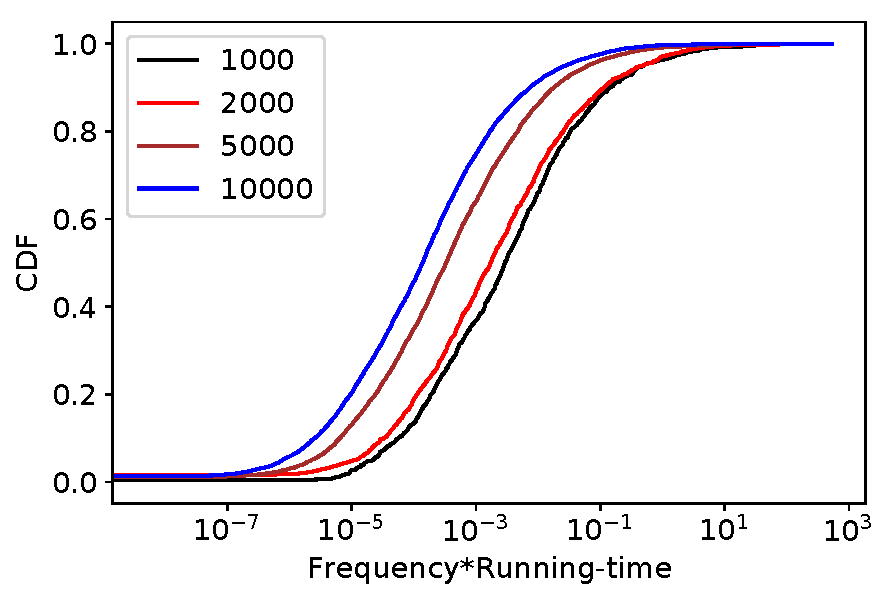
\includegraphics[width=0.35\textwidth]{../figs/freqs-all.pdf}
    \vspace*{-0.2cm}
  \caption{Function load is very heavy tailed (note the log X axis). Each line represents a different random subset and associated subset size from the Azure function trace. }
  \label{fig:freqs}
    \vspace*{-0.2cm}
\end{figure}

For locality-sensitive load-balancing techniques to be effective it is important for each function to impose roughly similar load on the system. 
However, functions vary widely in their frequency of invocation as well as their running time. 
The running-time heterogeneity of functions can be seen in Table~\ref{tab:func-times}, which shows that the times can range from 100ms to almost one minute.
Thus, the computing requirements (in terms of running time) of functions is highly heterogeneous. 

The popularities of the functions (i.e., their invocation frequency) is also highly skewed. 
Figure~\ref{fig:freqs} shows the distribution of the frequency$\times$running-time, for four randomly sampled subsets of functions from the Azure trace. 
This metric is effectively the ``induced-load'' of a function. 
We see that the functions are extremely heavy tailed in their induced-load: the ``heavy'' top 20\% functions consume 2 orders of magnitude more resources than the average. 
Thus, with classic consistent hashing the servers handling the heavy functions will be extremely overloaded, which will contribute to severe function slow-down due to resource contention on the servers. 

\vspace*{-0.2cm}
\subsection{Bursty Invocations}

The second challenge is that the function arrivals can be very bursty and can vary widely by function. 
Figure~\ref{fig:iats} shows the inter-arrival-time (IAT) distribution computed from the Azure dataset.
We see the average IAT of functions varies widely (the ``All'' line in the figure): by more than seven orders of magnitude.

Importantly, the IAT of the popular functions (ordered by number of invocations) can be significantly lower and different. For instance, for the top 10\% of the popular functions, their $90^{th}$ percentile IAT is less than 1 second. In contrast, the $90^{th}$ percentile IAT for all functions is 2,000 seconds.
%
This heavily skewed workload also has significant ramifications for Load Balancing, since we must be able to handle highly bursty functions, as well as the long tail of infrequently invoked functions.
This fairness in function handling is thus an important challenge in FaaS Load-Balancing. 


\begin{figure}
  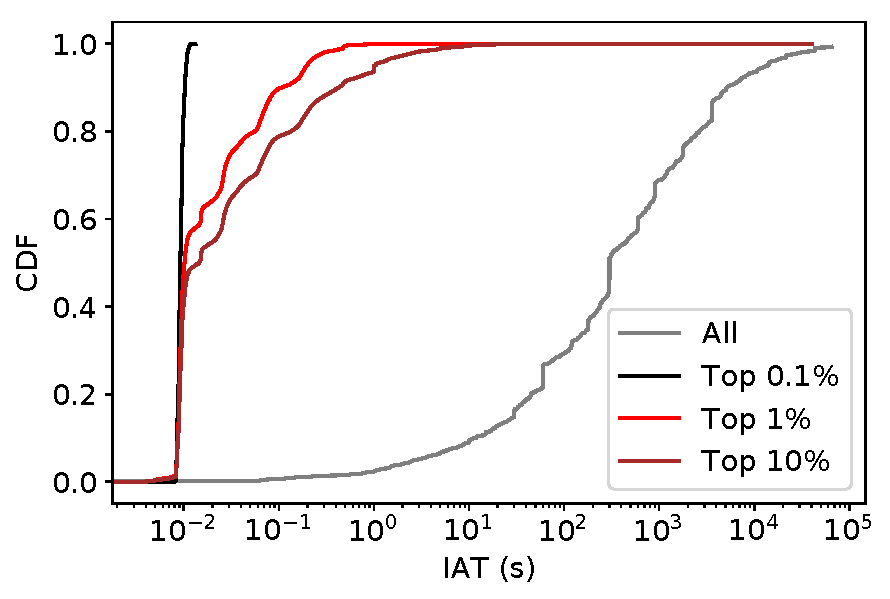
\includegraphics[width=0.35\textwidth]{../figs/iats-all.pdf}
    \vspace*{-0.2cm}
  \caption{Inter arrival times of popular functions can be extremely low, and show a very wide variance (note the log-scale of the X axis).}
  \label{fig:iats}
  \vspace*{-0.2cm}
\end{figure}

\vspace*{-0.2cm}
\subsection{Function Performance and Server Load}
\label{subsec:function-perf}
% Here or next section?

Our goal is to minimize the total end-to-end function execution latency. 
Unlike classic data-oriented load-balancing, function execution latency can be highly sensitive to the server load.
That is, running on an overloaded server (even if it is a warm-start), can result in significant latency increase and performance degradation.

Function performance can be affected by many factors such as the number of concurrently running functions, the CPU utilization, the load-average, interference due to other colocated functions, etc.
The slowdown in a processor-sharing system due to system load has been well modeled.
Queuing theory approaches for G/G/PS systems approximate the running time of a task to be proportional to $1/1-\rho$, where $\rho$ is the system utilization/load.

However, function heterogeneity and their execution characteristics presents many challenges in modeling and understanding their performance.
We have found that the container initialization and other OpenWhisk overheads, \emph{even for warm starts}, can be a significant source of latency, slowdown, and jitter. 

% \begin{table}
%   \begin{tabular}{ c c c c }
% \hline
%   Application & Min Time (s) & Mean Time (s) & $99^{th}$ Pctl (s) \\ 
% \hline
%   Web-serving & 0.015 & 0.408 & 1.049 \\  
%   ML Inference (CNN) & 0.166 & 0.405 & 2.299 \\
%   Disk-bench (dd) & 0.016 & 1.123 & 2.534 \\  
%   % float & 0.014 & 0.148 & 1.026 \\  
%   % gzip & 0.014 & 0.157 & 1.065 \\  
%   % image & 0.014 & 0.213 & 2.697 \\  
%   Matrix Multiply & 0.013 & 0.159 & 1.054 \\  
%   Sklearn Regression & 0.15 & 2.32 & 11.06 \\  
%   AES Encryption & 0.015 & 0.171 & 1.221 \\  
%   Video Encoding & 0.15 & 1.138 & 9.96 \\  
%   JSON Parsing & 0.015 & 0.159 & 1.012 \\
% \hline
% \end{tabular}
% \caption{The system overhead on warm invocations for the functions from Table~\ref{tab:func-times} are surprisingly high, up to several seconds in the worst case. Times were taken under load from our experiments described in Section~\ref{sec:policy-comare}. }
% \label{tab:overhead-times}
% \end{table}


\noindent \textbf{Function Jitter.}
To understand how system conditions can affect runtime of our functions, we first track their end-to-end latencies while the system is empty. 
In Figure~\ref{fig:UnstableEmpty} run each function repeatedly until we have 15 warm runs, then normalize those warm times by the minimum run and plot the results as a violin.
Surprisingly most of our functions have wildly inconsistent runtimes, ranging from 2x to 20x!
OpenWhisk traverses a complicated code path with several network hops in order to run user code, even on a warm start. 
% We describe the path briefly here to demonstrate where the varied latencies are coming from:
% \begin{enumerate}
%   \item An invocation enters system and is routed to a server
%   \item A container is chosen and arguments are sent to it
%   \item The results are stored in an external in-memory database
%   \item The load balancer is informed of completion
%   \item It must retrieve the results from the database
%   \item Results are finally returned to the user
% \end{enumerate}
We recorded the minimum time for all this OpenWhisk overhead to be $0.015$ seconds, the \emph{average} was a shockingly high 0.5 seconds, and the $99^{th}$ percentile reached 5 seconds. 
These high system overheads are largely caused by write-contention on the shared databases OpenWhisk maintains for tracking functions and their results. 
% The few that are stable are long-running and CPU bound, performing video and image transcription or ML workloads.
This instability most strongly affects short running functions, but negatively affects everything in the system.
Such significant jitter motivates our stale-load aware load balancing policy, which we develop in the next section. 

% 1) load balancing bit, send to invoker
% 2) find container in pool
% 3) send args to container
% 4) put result in CouchDb
% 5) Inform controller/LB that func is done
% 6) retrieve result from LB
% 7) return to user

% Min:0.015, Avg: 0.5s, p99: 5s 

\begin{figure}
  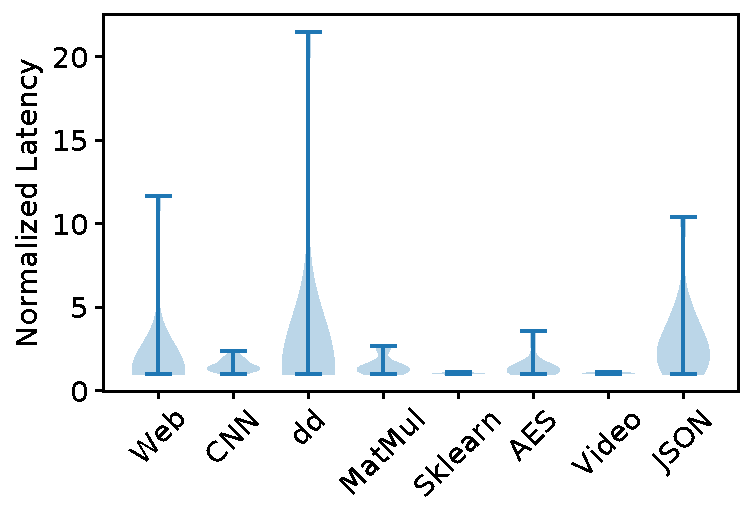
\includegraphics[width=0.33\textwidth]{../figs/ow/function_breakdown_min.pdf}
  \vspace*{-0.25cm}
  \caption{Functions warm latency has huge variance even under no system load, due to OpenWhisk jitter.}
  \label{fig:UnstableEmpty}
    \vspace*{-0.25cm}
  %XXX:Y Axis: Normalized latency
\end{figure}


% We also place the system under some load and examine how much of the end-to-end latency is spent in non-function computation.
% All functions, listed in Table~\ref{tab:overhead-times}, have a similar minimum overhead time of over one-hundreth of a second.
% While this is a significant time, the median times are all an order of magnitude higher.
% Fully half of function invocaitons spend a tenth of a second -often much more- stuck in the OpenWhisk pipeline.
% The baseline overhead time comes from the composite services of OpenWhisk communicating to invoke each function.
% Some of the more severe times we examined had the invoker waiting several seconds trying to inform the controller of a completed execution.
% The significant jitter encourages the use of a stale-load aware load balancing policy that is agnostic to such jitter.
% These forms of jitter mean that we cannot have an ``optimal'' load balancing policy from a latency perspective, as too many external variable affect a function's end-to-end latency.


\noindent \textbf{Load-sensitivity.} 
Furthermore, we have found that \emph{different functions are affected by server load differently.}
%
Figure~\ref{fig:LatencyVsLoad} shows the correlation between function latency and the Linux load-average of the server for different function types. 
The load-average is normalized to the number of CPU cores: thus a load-average of 2 in the figure for the 16-CPU VMs corresponds to a Linux load-average of 32.
The load on the servers was increased by increasing the number of concurrently executing functions of the same type.


We see that in general, as the server load increases, so does the latency of the function invocations.
Each point in the scatter-plots of Figure~\ref{fig:LatencyVsLoad} represents a unique invocation, with the latencies normalized to the lowest execution latency observed for that function.

The AES encryption function (Figure~\ref{fig:AES}) shows a gradual increase in latency as the load increases.
Surprisingly, the effect of load is minimal: the latency increases by ``only'' 2x even at a 10x load. 
%Nevertheless, does get affected by load, but surprisingly only under extreme cases where load is over 5!
The longer-running ML training function (Figure~\ref{fig:TRAIN}) also sees a correlation between server load and its end-to-end latency.
However, it's latency variance is lower because the longer running time (50 seconds) hides the variable OpenWhisk overhead.
Both functions presented here have the highest correlation between system load and latency, yet themselves do not have a high correlation.
Thus scheduling on an overloaded server can degrage function performance, it must be weighed against the performance penalty of a cold start.
% We describe this OpenWhisk ``system overhead'' more in Section~\ref{sec:unstable-latency}.
% Thus, running warm functions on overloaded functions comes with performance degradation risk, which is highly variable and hard to model, which presents yet another load-balancing challenge. 

%Note that while it's worst-case latency was 1.6 times the ideal, that represents an additional \emph{30 seconds} until it completes.
% \textbf{Alex: Earlier text said TRAIN had high correlation. But it doesnt (axes are not the same). It only shows less variance.}
%Certain functions see essentially no impact from server load, such as the web-server in Figure~\ref{fig:CHAM}, because they do not use much CPU or have extended runtimes.


\begin{figure}
  %\subfloat[]{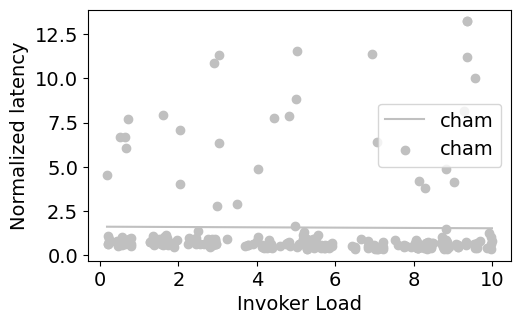
\includegraphics[width=0.22\textwidth]{../figs/lat-under-load/filtered/latency_to_load-loadAvg-cham.png} \label{fig:CHAM}}
  \subfloat{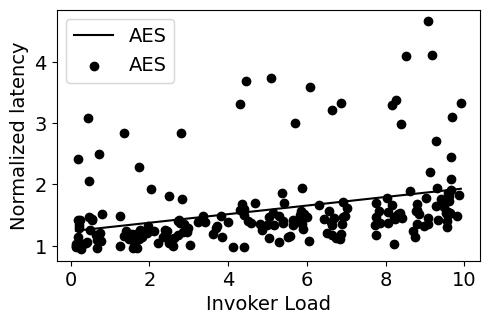
\includegraphics[width=0.22\textwidth]{../figs/lat-under-load/filtered/latency_to_load-loadAvg-aes.png} \label{fig:AES}}
  \subfloat{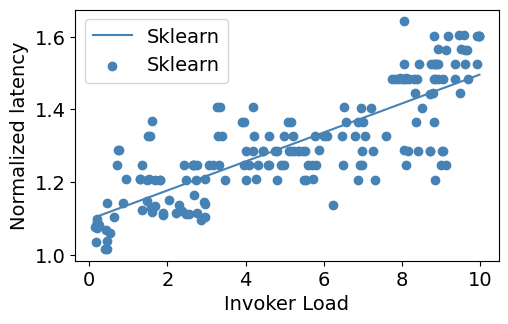
\includegraphics[width=0.22\textwidth]{../figs/lat-under-load/filtered/latency_to_load-loadAvg-train.png} \label{fig:TRAIN}}
    \vspace*{-0.25cm}
  \caption{Latency increases due to system load, but is function-dependent.}
  \label{fig:LatencyVsLoad}
  \vspace*{-0.25cm}
\end{figure}


% CH with bounded loads is a good idea, but 
% In a large cluster, cant assume perfect load information, which is especially challenging for
% Stale loads (Dahlin) and follow-up work: homogenenous requests making it easy to predict what the server load is going to be based on the number of requests sent. But not applicable here. 




%%% Local Variables:
%%% mode: latex
%%% TeX-master: "paper"
%%% End:


% case for priorities?

\section{Function Prioritization Motivation}
\label{sec:qos:motivation}

\begin{table}
  \caption{Delay-tolerant scenarios. The ID of the use case is taken from a public dataset~\cite{Eismann:zenodo:2021:dataset}. We studied each case and estimate a likely delay tolerance for that scenario.}
  \label{tab:examples}
  \centering
  \begin{tabular}{lrlp{0.6\linewidth}}
    \hline
    Trigger group & ID & Delay     & Description \\
                  &    & tolerance & \\
    \hline
    timer & 6 & $<$10min & NetApp's cloud function to periodically find unutilized EBS volumes to delete. \\
    event & 28 & $<$60min & Google Analytics clone to track website visitors. \\ %Note from Cristina: Google Analytics updates statistics every 24-48 hours for standard accounts 
    queue & 59 & $<$60min & Messenger Chatbot for a media company; sends weekly news updates to user. \\
    storage & 30 & $<$10min & Serverless Galleria, for batch manipulation and publishing of images. \\
    orchestration & 12 & $<$24h & Subscription fulfillment for online and print subscriptions of The Guardian. \\
    others & 101 & $<$10min & Scientific task, batch, on demand, for sequence alignment of protein sequences. \\
  \hline
\end{tabular}
\end{table}

In this section, we show that---in opposition to what others have argued in the past~\cite{Wiesner:Middleware:2021:TemporalShifting}---(some) real serverless workloads \emph{are} delay tolerant (Section~\ref{sec:motivation:delay-tolerant}), we discuss the current status of differentiated serverless functions (Section~\ref{sec:motivation:currentStatus}) and provide a workload characterization based on dividing functions into high- and low-priority classes (Section~\ref{sec:motivation:workload}).
Our study of the delay tolerance of serverless functions is based on a recent dataset of serverless applications~\cite{Eismann:Software:2021:Why,Eismann:TSE:2021:CommunityConsensus}.
For the workload characterization, we analyze traces with real serverless workloads from Microsoft Azure~\cite{shahrad2020serverless} and present the results of one representative day (day 5 of the 2-week trace).
%we have released the code used for the analysis in this section.\footnote{GiHub link blinded for review.}

\subsection{Can Serverless Functions be Delayed?}
\label{sec:motivation:delay-tolerant}
In this subsection, we analyze if serverless functions can tolerate some level of delay in their execution. 
This delay could come from not executing the function immediately (e.g. through queuing), or via reduced priority in scheduling (e.g. giving less resources to lower-priority functions).
While these two mechanisms differ, the result of both is increasing the turnaround time of the functions; this increase is not appropriate for some functions---like those supporting interactive or real-time applications---but is tolerable for multiple other applications, as discussed in this subsection.

Serverless functions can be triggered through several mechanisms like http invocations, cloud-native events, queue messages and timers.
Functions triggered by http are time sensitive as these are synchronous requests that can timeout and are often used in interactive applications;
all other triggers invoke functions that can tolerate delays to varying degrees.
Thus, functions not triggered by http are (potentially) delayable; in the Azure trace, these constitute $59.06\%$ of the functions and $69.07\%$ of the invocations.

Furthermore, a recent survey of serverless use cases~\cite{Eismann:TSE:2021:CommunityConsensus} found that 66\% of applications in a large dataset have at least one delay-tolerant function.
To further illustrate our point, we analyzed the applications in the dataset and selected one delay-tolerant scenario for each of the triggers (except http, which is not delayable as already explained);
these scenarios are described in Table~\ref{tab:examples} and include examples such as removing unutilized EBS volumes, a web analytics (clickstream) application, a messenger chatbot, a batch image manipulation application for a serverless galleria, a subscription fulfillment application for The Guardian, and an application for sequence alignment of protein sequences.

A note on http-triggered functions: Some web applications need end users to invoke asynchronous behavior via http requests.
The Microsoft Azure Cloud Design Patterns documentation~\cite{Eastbury:2022:Azure:AsyncPattern} provides a solution to this problem with the ``Asynchronous Request-Reply'' pattern which disaggregates such behavior into three functions: two http-triggered ones (to enqueue request and to check status of job), and a queue-triggered backend function.
In this scenario, the http-triggered functions are not delay tolerant, but the queue-triggered function is.
%(though it may tolerate only a small delay depending on the specific use case).


\subsection{Current Status of Differentiated FaaS Invocations}
\label{sec:motivation:currentStatus}
A recent empirical study~\cite{Tariq:SOCC:2020:Sequoia} found that current cloud providers (AWS, Azure, GCP and IBM) treat http functions differently from those triggered by other means, frequently via undocumented behavior, including different concurrency limits and prioritization versus background functions.
In addition, while asynchronous functions are queued and thus the user understands that they may not execute immediately, providers don't typically enqueue synchronous functions but rather return with an error if peak exceeds concurrency limits or provider capacity.\footnote{An exception is GCP which handles synchronous calls in best effort fashion, performing queuing but not ensuring zero drops~\cite{Tariq:SOCC:2020:Sequoia}.}
%
Thus, the major public cloud providers are already implicitly defining two classes of functions: high priority (synchronous) and lower priority (asynchronous), with the latter being delay-tolerant.
%asynchronous functions in AWS can be queued up to 6 hours.\footnote{\url{https://docs.aws.amazon.com/lambda/latest/dg/invocation-async.html}}
%Asynchronous functions are either explicitly (for example, with the \texttt{async} keyword in OpenWhisk) or implicitly (by its trigger) defined in current platforms.
%The asynchronous functions are good candidates to be delayed if needed.

In OpenWhisk asynchronous functions are defined with the \texttt{async} keyword and follow a different execution path than synchronous ones.
However, the platform does not use any mechanism to delay or execute them at a lower priority.
A solution that treats \texttt{async} functions as delay-tolerant, scheduled with a lower priority than synchronous functions, can be added to OpenWhisk without API modifications.

\subsection{High- and Low-Priority Workloads}
\label{sec:motivation:workload}
%Re-write section: try to make more compact 1-2 paragraphs is better
Considering the two function classes described in the prior subsection---high and low priority---we analyze the Azure traces applying this division in the workload.
For the high priority class, we consider http-triggered functions.
For the low priority class, we consider all other functions.

%\paragraph{Prevalence in workload}
High-priority functions constitute a significant portion of the workload, though the low-priority functions are greater in number and account for more than 2/3 of the invocations.
Specifically, high-priority functions constitute $41\%$ of the functions and $31\%$ of the invocations, versus $59\%$ of the functions and $69\%$ of the invocations for the low-priority.
%Higher precision numbers:
%$40.94\%$,  $30.93\%$
%$59.06\%$, $69.07\%$ 

%\paragraph{Function duration}
Figure~\ref{fig:CDF:workload} (Left) shows the cumulative distribution function (CDF) of the average function durations.
%; the dataset does not contain the duration of each invocation, just per-function aggregate statistics.
The function durations are similar for both classes, with high-priority functions being slightly shorter (median 0.2 vs 0.8 minutes).
%\paragraph{Interarrivals}
Figure~\ref{fig:CDF:workload} (Right) shows the CDF of the per-function average inter-arrivals;
%The dataset contains arrivals aggregated at per-minute intervals, making it impossible to get low granularity statistics for interarrivals smaller than one minute; most (98.8\%) interarrivals fall in this category.
the IATs for both classes are similar.
%---at the granularity that we can do the analysis---

% \begin{figure}[t]
%     \centering
%     \includegraphics[width=0.8\columnwidth]{../Figures/CDF-functionDurationsByPriority.eps}
%     \caption{CDF of the function durations, with functions divided into two groups: high-priority and low-priority.}
%     \label{fig:CDF:durationByPriority}
% \end{figure}

\begin{figure}[t]
    \centering
    \begin{minipage}{0.49\linewidth}\vspace{0pt}%
        \includegraphics[width=\linewidth]{chrlu/qos/Figures/CDF-functionDurationsByPriority.eps}
    \end{minipage}
    \begin{minipage}{0.48\linewidth}\vspace{-5pt}%
        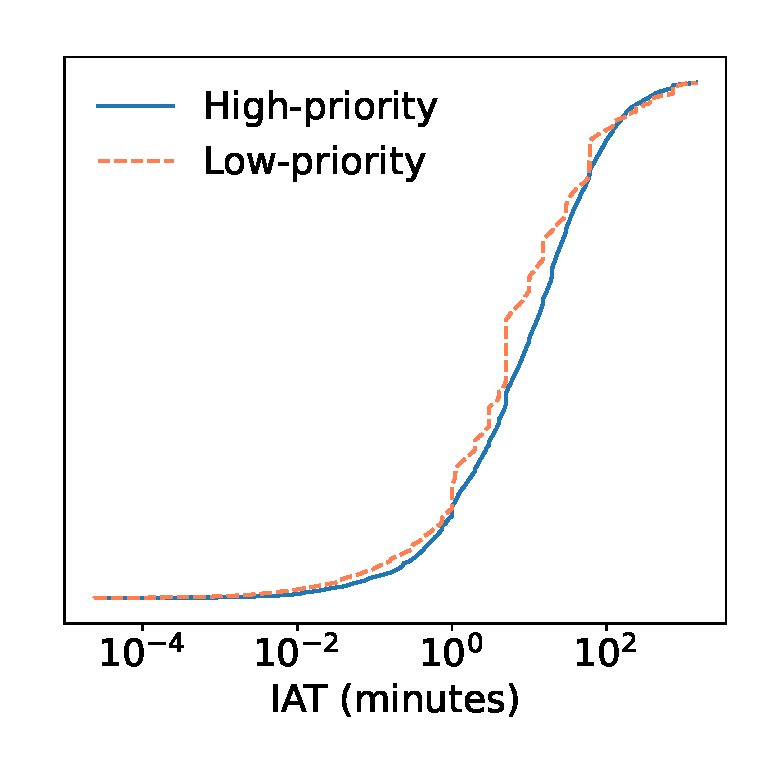
\includegraphics[width=0.95\linewidth]{chrlu/qos/Figures/CDF-averageInterarrivals.eps}
    \end{minipage}
    %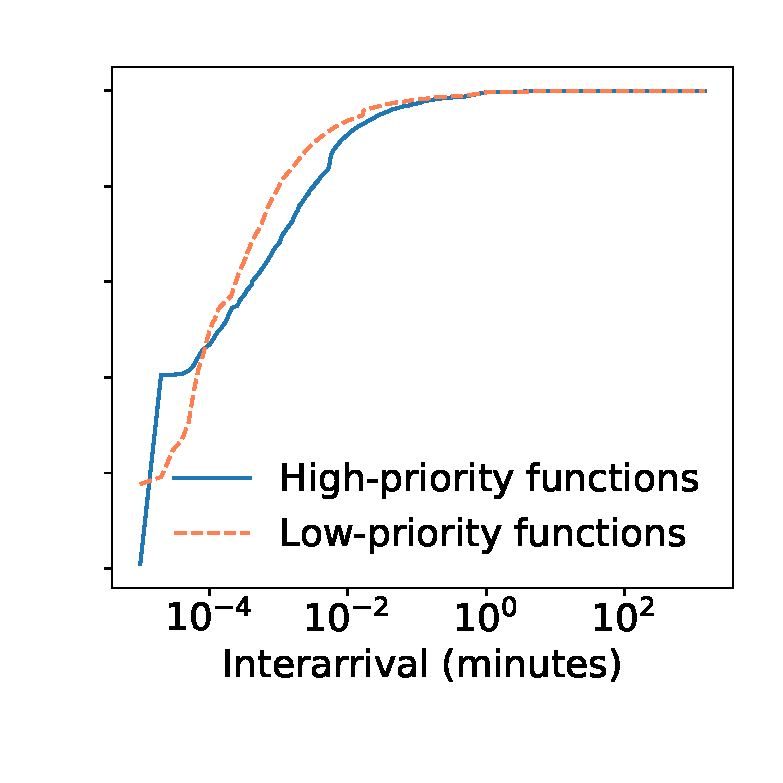
\includegraphics[width=0.49\columnwidth]{../Figures/CDF-interarrivals.eps}
    \caption{Left: CDF of the function durations. Right: CDF of the average function inter-arrivals. Functions are divided into two classes: high and low priority.}
    \label{fig:CDF:workload}
\end{figure}


% \begin{figure}[t]
%     \centering
%     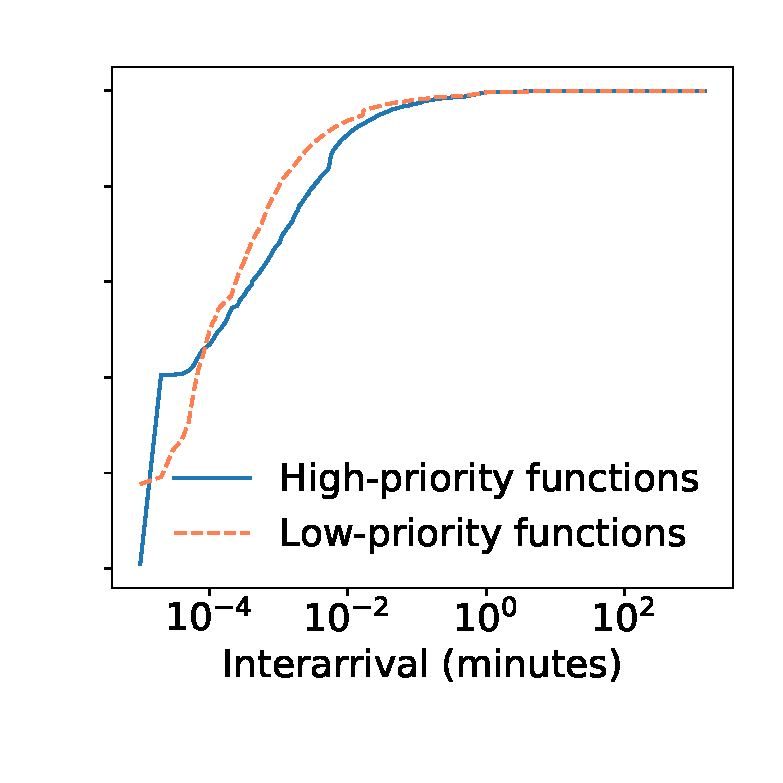
\includegraphics[width=0.8\columnwidth]{../Figures/CDF-interarrivals.eps}
%     \caption{CDF of the per-function interarrivals, with functions divided into two groups: high-priority and low-priority.}
%     \label{fig:CDF:interarrivalsByPriority}
% \end{figure}

\begin{comment}
\paragraph{Burstiness}
Figure~\ref{fig:bursty:highVsLowNormalized} shows the per-minute invocations, with functions divided into high and low priority groups and with invocations normalized to their peaks.
Both groups have similar burstiness: high-priority ($IDC=0.0083, \sigma=0.0794$) and low-priority ($IDC=0.0079, \sigma=0.0764$).
Even though the burstiness is similar, the peaks may or may not align during the 24-hour period.

\begin{figure}[t]
    \centering
    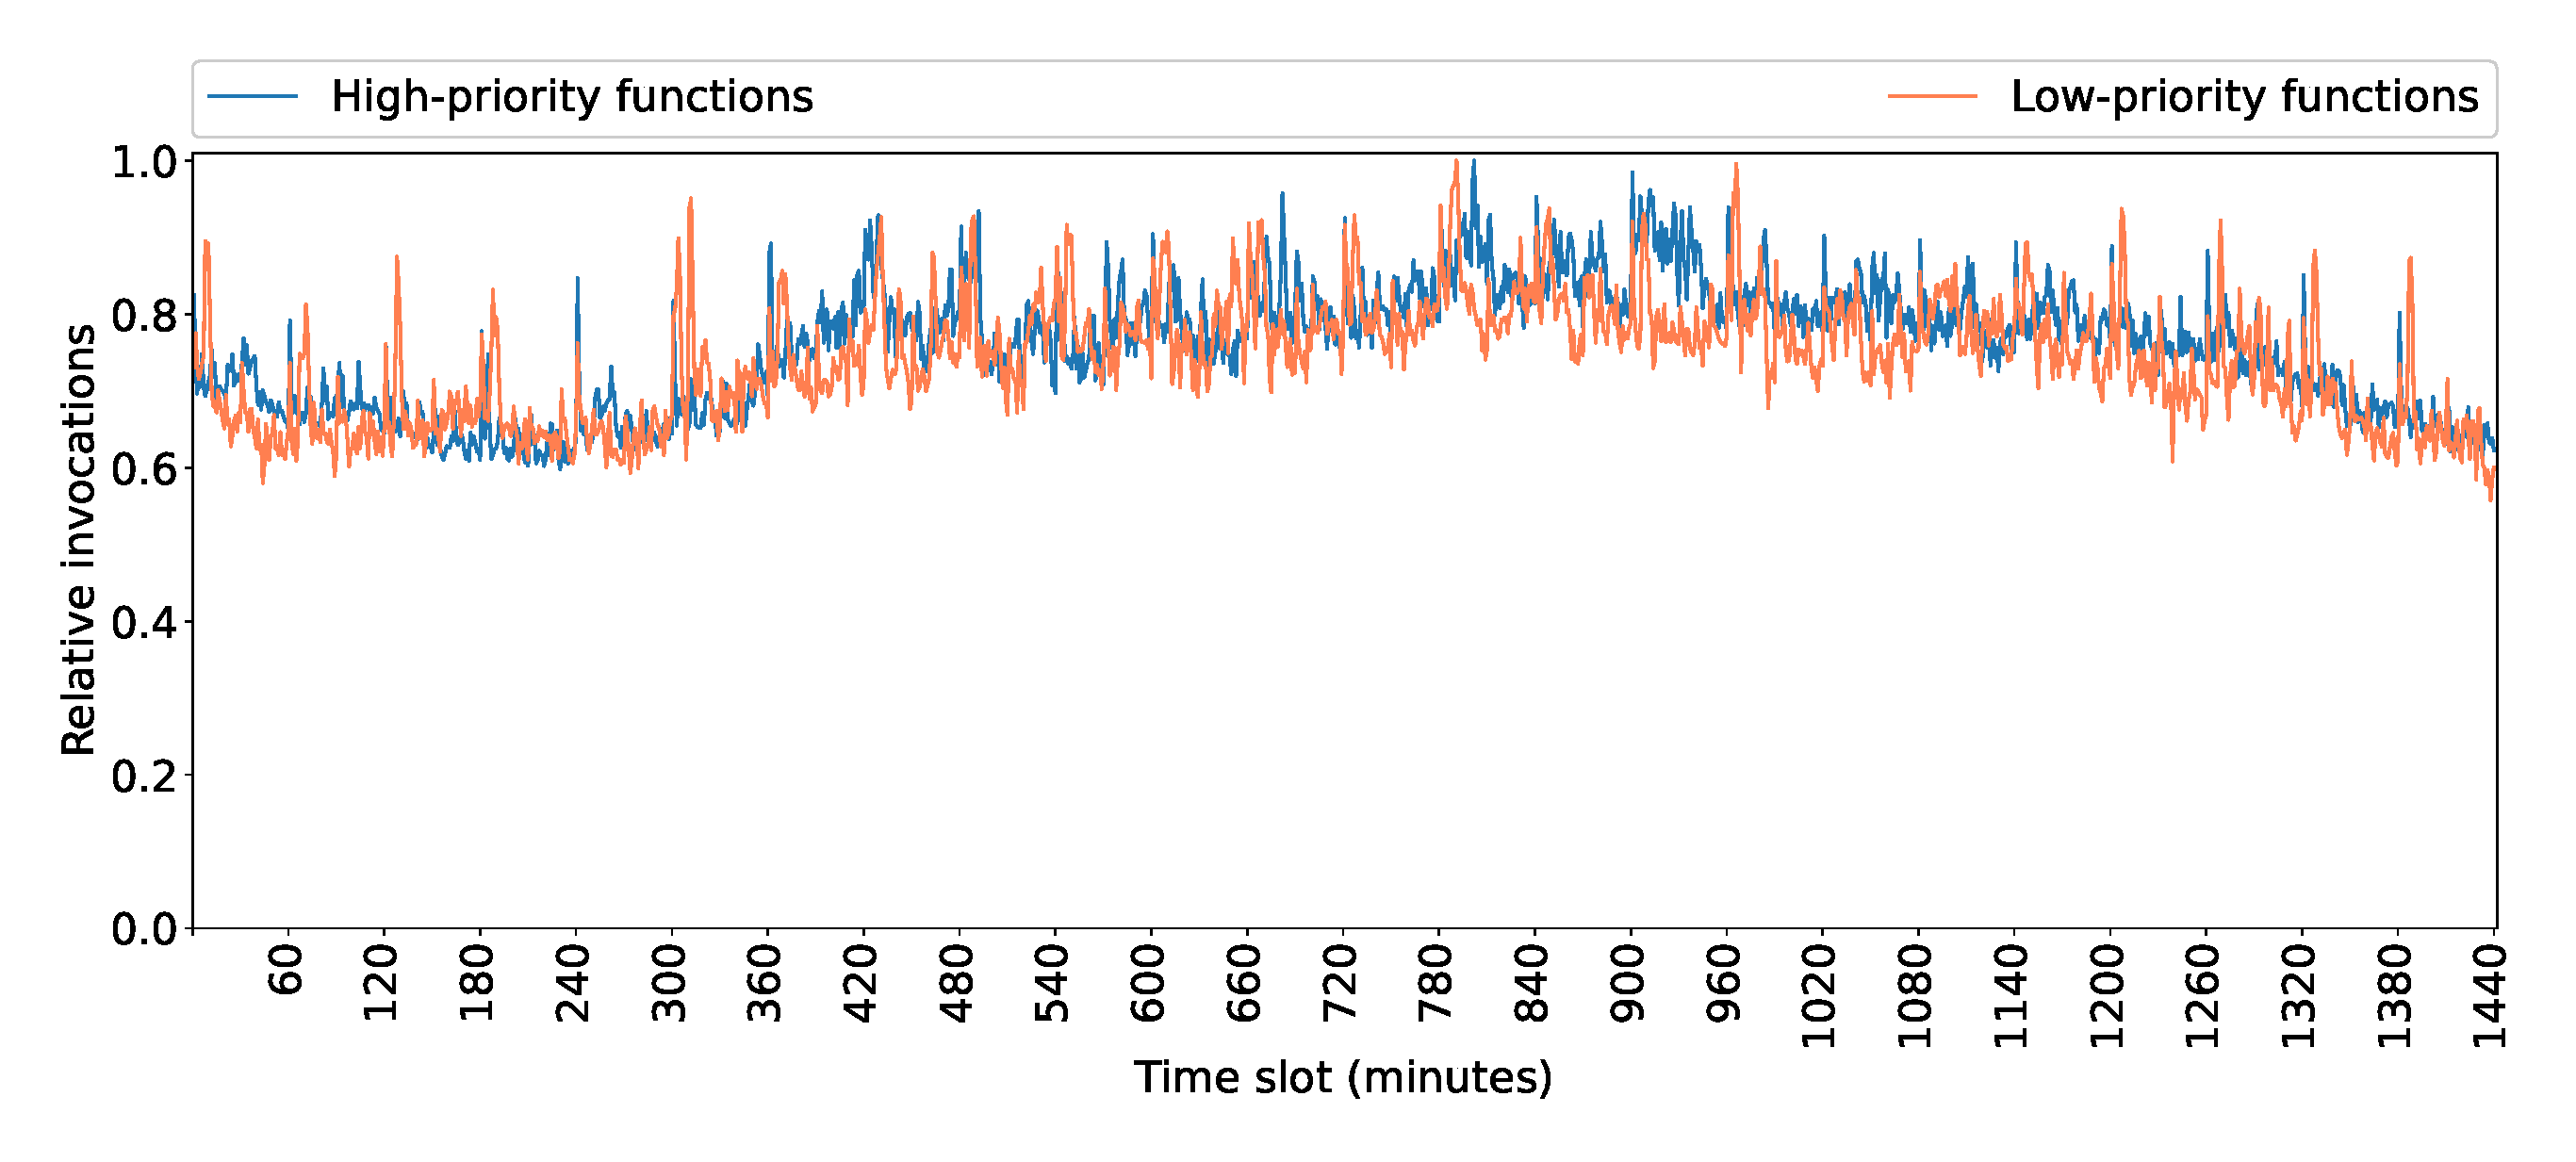
\includegraphics[width=\columnwidth]{../Figures/bursty-HighVsLowNormalized.eps}
    \caption{Invocations per minute, normalized to their peak, with functions divided into high- and low-priority groups.}
    \label{fig:bursty:highVsLowNormalized}
    % High-priority functions: 
    %   standard deviation :  0.0794
    %   IDC:  0.0083
    % Low-priority functions: 
    %   standard deviation :  0.0764
    %   IDC:  0.0079
\end{figure}
\end{comment}


%%% Local Variables:
%%% mode: latex
%%% TeX-master: "paper"
%%% End:


\section{Priority Based Consistent Hashing} % Based Load Balancing Policies}
\label{sec:qos-chrlu}

In this section, we extend the load-balancing algorithm to take into consideration function \emph{priority}, in addition to the characteristics in Section~\ref{sec:chrlu}. 
% We assume a cluster of homogeneous servers, and that a new function invocation can be sent to any of the servers.
% Each server implements keep-alive for functions: after successful execution, the function's container is stored in server memory, and evicted based on some eviction policy.

\begin{figure}
\centering
  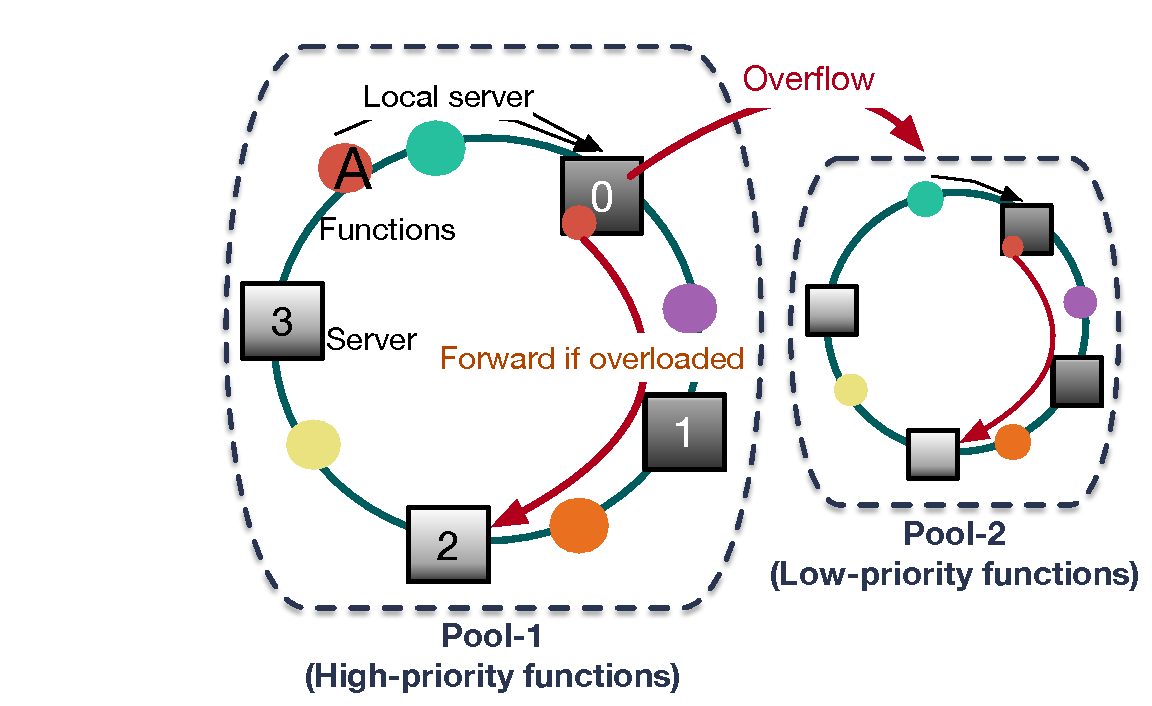
\includegraphics[width=0.8\textwidth]{chrlu/qos/figs/k-rlu2.pdf}
  \caption{$k$-CH-RLU partitions a cluster into multiple server pools and runs server-load-aware consistent hashing in each pool. Functions are forwarded if servers are overloaded, or to a lower-priority pool if the entire pool is.}
  \label{fig:2-pool-arch}
\end{figure}

% Overview of the architecture. 
\subsection{Quality of Service Architecture}

To support quality of service (QoS) for functions of different priority levels, we use a two-stage load-balancing architecture (see Figure~\ref{fig:2-pool-arch}). 
The cluster is partitioned into multiple pools, one for each priority level.
For ease of exposition and without loss of generality, we consider two levels: high- and low-priority functions, and thus two corresponding pools. 
Within a single pool, functions are load-balanced among servers using a load-aware consistent hashing technique. 
Our approach is modular: each pool runs an independent load-balancing policy, which is the focus of most of this section. 
This approach also preserves function locality, which is important for reducing cold-starts, as we describe next.  

\subsection{$k$-CH-RLU}
\label{subsec:kchrlu}

Our overall policy, Consistent Hashing with Random Load and Updates with $k$ pools ($k$-CH-RLU), combines all the previously described techniques and insights.

Upon a new function invocation, it runs in its pool using the \texttt{forward} procedure in Algorithm~\ref{algo:PopularRLUPolicy}, which combines the use of SHARDS for popularity detection, cold and warm times for increasing the effective load bound, and noisy loads. 
The initial server is determined using a consistent hashing function. 
We bound the cold/warm ratio with a final load upper bound, $b\_max$.
The load-bound parameters determine the locality sensitivity: higher values of $b$ and $b\_max$ increase locality at the risk of resource-contention delays.
Similarly, higher values of $p$ results in more aggressive random forwarding and reduces locality. 

Our two-level architecture is modular and allows us to parameterize different load-balancing policies for different pools.
Lower-priority pools are run with a higher load bound $b\_max$, and thus tolerate more overloaded servers, at the risk of lower function performance.
Forwarding along the chain has diminishing returns on locality, and if the function gets forwarded more than $max\_chain\_len$ times, it triggers the overflow condition.

Function prioritization and QoS are controlled via the server pools: Each function has a default pool based on their priority level, with higher-priority functions having lower pool numbers. 
The high-priority functions recursively overflow to the next lower-priority pool, and thus have good locality because all pools use our consistent hashing approach. 
The high-priority functions can thus overflow and potentially use the entire cluster in case of workload spikes, preserving their QoS. 
The lower-priority pools thus also serve as a ``burst buffer'', crucial considering the bursty nature of functions. 
Low-priority functions can't make use of higher-priority servers even if they are available, since we want to be able to handle bursty invocations of higher-priority functions. 
For the lowest-priority pool, we run the function on the least-loaded server in their pool. 
%
If the least loaded server is also overloaded, we drop the function.
% \begin{figure}
% \begin{algorithm}[t]
%   \caption{$k$-CH-RLU}
%   \begin{algorithmic}[1]
%     \Procedure{forward}{$pool, func, server, chain\_len $}
%     \State $b, b\_max, max\_chain\_len \gets system\_params $
%     \If{$ chain\_len > max\_chain\_len $} \Comment Overflow 
%     \If{$ pool == k $} \Comment Lowest-priority pool
%     return least-loaded-server
%     \Else \State forward(pool+1, func, server=CH(func, pool), 0) \Comment Try in next pool 
%     \EndIf 
%     \EndIf 

%     \State $\lambda \gets 1.0 / avg\_iat$ \Comment Computed from Algo 1
%      \State $L=Load(server)$
%     \If{popular(func)} \Comment Computed from Algo 1 
%          \State $L = Load(server) + \mathcal{N}(\mu=\lambda\,\sigma=0.1)$
%     \EndIf 
%     \If{$L < min(cb/w, b\_max)$}
%        \State server
% \Else \State forward(pool, func, next(server), chain\_len+1)
%        \EndIf
%        \EndProcedure
%     \end{algorithmic}
% \label{algo:PopularRLUPolicy}
% \end{algorithm}

% \begin{algorithm}
  
% \end{algorithm}



\noindent \textbf{Pool Sizing.}
The priority pools are sized proportional to the number of functions registered at different priority levels.
Thus, if 25\% of all functions are low-priority, then 25\% of the servers are in the low-priority pool and the rest are in the high-priority pool.
Periodically, we recompute this ratio based on the currently registered functions, which may lead to resizing the pools.
Importantly, locality is preserved even after pool resizing because of consistent hashing. 


\begin{comment}
We have also implemented a simple PID controller with hysteresis for horizontal scaling, by using server load averages as the input control signal. 
This horizontal scaling is conservative, with a large dead-band of 5 minutes, and scaling is triggered only if the at least 50\% of the servers are overloaded.
As we shall show in the empirical evaluation, CH-RLU significantly reduces the variance in the loads among servers, and thus is more amenable to this horizontal scaling policy. 
\end{comment}


% Unpopular functions still use Algorithm~\ref{algo:ConsistentCachePolicy}.
% In all cases, if we exhaust the list of servers trying to find one with low load, we randomly assign the invocation to a server.
% This only occurs in the most extreme cases of system load and also prevents spamming a popular server in that same scenario.



% if popular: L+Noise > bound 
% else: L > bound 

%%% Local Variables:
%%% mode: latex
%%% TeX-master: "paper"
%%% End:


%\section{QoS Policy}

Users provide the QoS priority. Currently binary: high and low priority. 

\subsection{QoS Policy Tradeoffs and Challenges}

There are many possible paths towards realizing QoS differentiation on FaaS clusters, and we now discuss different possible approaches and their tradeoffs.

\paragraph{Cgroups.} We can enforce service differentiation at the \emph{server} level: and use the virtual environment's resource allocation and control mechanisms.
For instance, we can use cgroups to reduce the relative and absolute cpu and memory allocation of the low-priority function containers.
While this approach is feasible, it has some drawbacks.
Mainly, using cgroups only controls the resource footprint of the actual function execution.

However as we saw in the previous section, a significant, often majority, time is spent in the various function initialization steps.
This initialization is not necessarily part of the ``function context'', and thus not directly controllable through cgroups-like mechanisms.
Significant resource consumption occurs in initializing the function for cold starts and \emph{even for warm starts.}
Specifically, we found that unpausing a docker container and allocating network interfaces to it can consume significant CPU resources.

However, this resource consumption occurs as part of the FaaS ``control plane'', i.e., OpenWhisk, Docker, kernel components for networking, namespaces, and cgroups.
Using cgroups to reduce resource allocation by reducing the cgroup priority/quotas/limits only reduces function execution speed, but misses the significant (and often the majority) resource consumption in the control plane.
Thus,
\todocristina{Last paragraph is incomplete; other than that, we need a figure for the unpausing docker container experiment.}

\paragraph{Queueing at the server.}
Another server-level approach is to introduce a queue at each server, which can prioritize function execution by delaying low-priority functions.
This can be a  powerful approach in general.
Priority queueing algorithms often assume some deterministic or a probability distribution of service times of the different jobs such as exponential distributions.

However, function execution times, due to the control-plane overheads, show a very high variance, and their execution time is not exponentially distributed.
Moreover, function execution times are highly heterogenenous, and servers run 100s of different functions, which makes analytical solutions non-trivial. \todocristina{Do we know that function durations are not exponentially distributed?}

\textbf{Need to tighten this argument, or remove it.}

Server-level throttling either using cgroups or queueing also has more general tradeoffs. 
If all servers are available for a delayable function to use, then idle servers can be used to opportunistically run them. 
However, this may lead to poorer locality (i.e., more cold-starts), and increased risk of performance interference between high and low priority functions. 

% Our approach : 

\subsection{Our approach: Cluster Pools}

Key idea is to have a separate pool of servers for running the low-priority delayable functions. 
The high priority pool handles the conventional functions. 

Within each pool, we use a locality-aware load-balancing policy to reduce the effects of cold-starts and server loads. 

\subsection{Low priority pool as Burst buffer}

Low priority servers can be used to handle high priority invocations in case of bursty invocations that are quite common.

We integrate load balancing with cluster pools to handle workload bursts.

\begin{itemize}
\item Locality is important, so we must build on consistent hashing. 
\item However, consistent hashing alone results in overloaded servers because of the heavily skewed workload (1\% functions taking 90\% resources, etc.)
\item This is fixed with bounded loads and forwarding. Make sure each server has a max capacity. For a new invocation will exceed this capacity, it is forwarded along the ring. 
\item For bursty functions, even this may be suboptimal, since a sudden burst of invocations can saturate many consecutive servers, starving other functions of warm hits. 
\item Thus, recently, CH-RLU has been proposed: which adds a random load to each server for popular functions, to forward popular functions more aggressively. 
\item We build on CH-RLU. 
\item For forwarding functions, we set a max forward limit (the chain length). If we exceed the chain length, \emph{our key idea is to run the function on the low-priority cluster pool.} Currently, CH-RLU will run function on least-loaded server, breaking locality. 
\item Our key new idea also preserves locality. Popular functions likely to run on the same subset of servers in the low priority pool. 
\item Low-priority pool continues to use CH-RLU without any overflowing. 
\item Thus bursts can be quickly handled without slow and expensive repartitions. 
\item We call our policy ``CH-RLO'': Consistent Hashing with Random Loads and Overflow. 
\end{itemize}


\subsection{Partitioning Policy}

Assume we have a fixed number of servers, $S$. 
Out of these, $x$ are for the high-priority functions, and the remaining $S-x$ for the low-priority functions. 
The ultimate goal of the partitioning policy is to decide what $x$ should be. For this, we use a simple online control-based optimization approach. 

\textbf{Initial configuration.}
Since functions have to be registered as low or high priority, we set $x/S$ proportional to the ratio of number of high ($N_H$ )and low priority ($N_L$) functions.
Specifically, we introduce an overcommitment parameter $c$ that determines how small the low-priority pool is going to be.


\begin{equation} x_0 = c \frac{N_H}{N_L} S \end{equation}

\textbf{Adjusting x.}
Note that the invocation frequency and running time of functions can vary widely, so this initial assignment need not be ideal.
Our goal is to improve the performance of both the high and low priority functions, but deprioritize the performance of low-priority functions by a factor of $c$.
Thus, the objective function, $F$, is:
\begin{equation}
  F(x) = f_H - \frac{f_L}{c},
\end{equation}
where $f_H$ is some aggregate performance measure of all high-priority functions, and $f_L$ is for low-priority.

We use
\begin{equation}
f_H=\sum_i^{N_H} \frac{\bar{\tau_i}}{\min{\tau_i}},  
\end{equation}

where $\bar{\tau_i}$ is the average latency of function $i$. (Better symbol? L already used for Low priority). 
More concretely, the performance measure is the increase in latency. Since FaaS providers do not have access to the ``ideal'' or baseline latency, and because it can vary widely based on the function (from few ms to few minutes), it needs to be normalized. We normalize each function's latency by the minimum latency of that function observed so far. 

Our goal is to balance the cluster so that $F(x)=0$.

Thus, periodically, we use a gradient-based method: $\delta(x) = \eta F(x)$, where $\eta$ is the step size.

We can consider other objective functions too.
One appealing one is to measure the delay of functions explicitly, where delay is defined as the total latency minus the actual function execution duration. This captures the FaaS control-plane (i.e., OpenWhisk, docker and other components) overheads.



%%% Local Variables:
%%% mode: latex
%%% TeX-master: "paper"
%%% End:


%\vspace*{-0.2cm}
\section{Implementation}
\label{sec:impl}

We have implemented our consistent hashing with random load update (RLU) policy and other load-balancing policies in OpenWhisk, a popular FaaS system.
Our changes amount to more than 1,700 lines of code across many OpenWhisk components, but are primarily in the load-balancer class. 
In this section, we describe major implementation details, as well as key performance optimizations which significantly improve OpenWhisk performance and scalability by more than $4\times$. 

Our policies are implemented by modifying the load-balancer module of OpenWhisk (see Figure~\ref{fig:sys-diag}).
CH-RLU is implemented by modifying the existing OpenWhisk ``container sharding'' policy, which also uses consistent hashing, and forwards functions using only available memory as the load metric.
We use OpenWhisk's existing consistent hashing implementation, permiting an ``apples to apples'' comparison, and also making CH-RLU a ``drop-in'' replacement for the OpenWhisk default load-balancing. 
At the invoker level, we adapt FaasCache's GreedyDual keep-alive policy, which increases the keep-alive effectiveness compared to OpenWhisk's default non-resource-conserving TTL eviction~\cite{faascache-asplos21}. 

\begin{figure}  
  \centering
  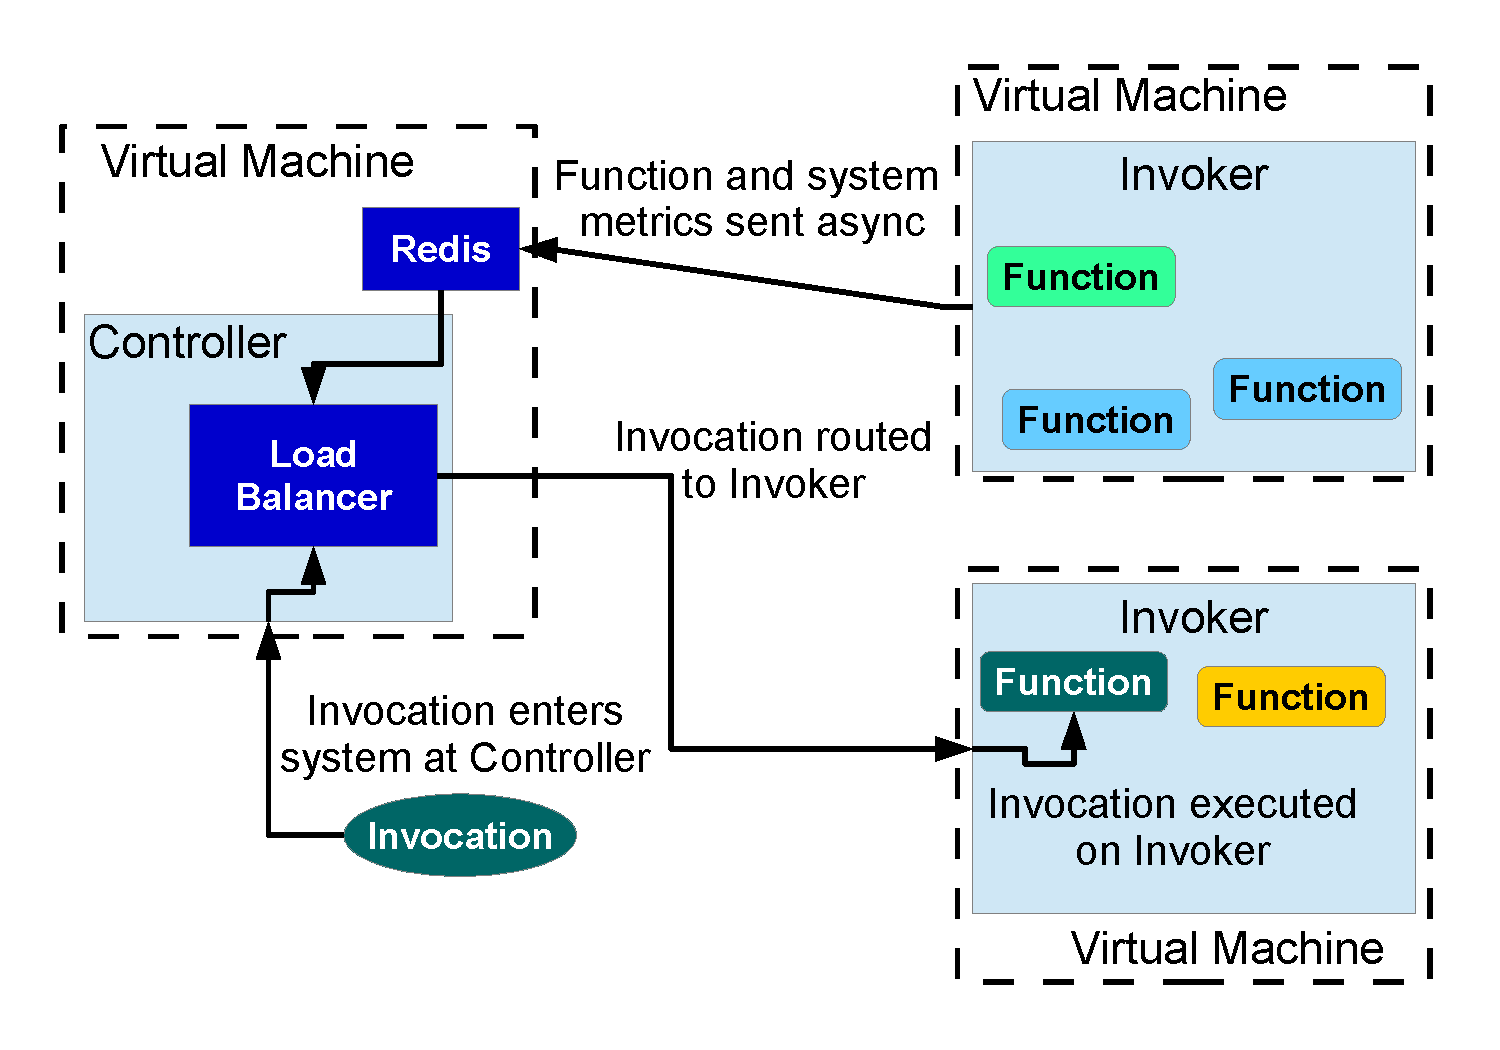
\includegraphics[width=0.6\textwidth]{chrlu/faaslb-osdi22/figs/sys-diag.pdf}
 %   \vspace*{-0.3cm}
  \caption{System diagram of relevant OpenWhisk components and communication used to schedule and run function invocations.}
  \label{fig:sys-diag}
  %  \vspace*{-0.3cm}
\end{figure}

The CH-RLU algorithm described in the previous section requires two main additional pieces of information from each invoker/server: the load averages, and the cold/warm running times of functions. 
Both of these are periodically (every 5 seconds) captured and stored in a centralized redis key-value store.
The load-balancer in the controller reads these asynchronously: working with stale and inconsistent metrics is our key design goal. 
The default load-bound, b, is 1.2, and the max load, b\_max is 6. Popularity threshold is set to 20\%.
We did not observe performance to be very sensitive to these parameters, and thus do not need to auto-tune them, and they are suitable as user-inputs. 

%\vspace*{-0.2cm}
\subsection{Performance Optimizations For OpenWhisk}

Since our goal is to run functions under high load, we ran into a large number of OpenWhisk performance and scalability bottlenecks.
We found default OpenWhisk to be almost unusably slow and unstable even under reasonable load. 
We present their details and our actions to overcome them, hoping that the fast-growing serverless computing research field can benefit from our lessons. 


In our experience, the primary source of scalability bottlenecks when concurrently managing Docker containers.
We found significant contention in \texttt{dockerd}, Docker's control daemon which handles all the container lifecycle events.
Even at moderate loads (normalized server load average close to 1), high dockerd contention can increase tail latencies by \emph{several minutes!}


Currently, OpenWhisk \textbf{pauses} each container after function execution, which prevents it from being scheduled by the CPU.
It then resumes the container before running the next invocation of the same function (assuming a warm start).
Each invocation therefore requires these two additional (pause/resume) events to be handled by dockerd, which results in significant lock contention.
Because of the FaaS programming model, the pausing is not necessary, since nothing in the container can run after a function has returned.
Therefore, we remove these redundant pause/resume operations to reduce dockerd contention.
This reduces the OpenWhisk overhead by 0.2 seconds \emph{per-invocation} on average.
More importantly, by reducing dockerd contention, we were able to run a much larger number of concurrent functions. 

An even larger source of scalability bottleneck is \textbf{network} namespace creation time.
Using the default bridge networking requires each invocation to create a new TUN/TAP network interface.
We found this to be a very expensive operation because of Linux network stack overheads (several 100 ms), and because of dockerd's userspace lock (futex) contention for its networking database. 
We found that as the \emph{historical} total number of containers launched grows, so does the size of the network-interface database.
Dockerd reads and updates this database under the critical section, and the larger database results in higher lock contention.
As a result, we were unable to use VMs/servers with more than 4 CPUs after 20 minutes of sustained load, since the dockerd contention resulted in many functions timing out (timeout was 5 minutes)! 

We sidestep this problem by not using bridge networking, but instead using Docker's \textit{host} network option and assigning each container a unique port on the host. 
Implementing the network change required updating the OpenWhisk runtimes used to wrap functions to monitor their specified port.
This change allowed us to run functions on larger invokers and under more sustained load, and eliminated most timeouts. 

Finally, after a certain request rate threshold, we found the default \texttt{nginx} OpenWhisk frontend would crash and return \textit{502 BAD GATEWAY} for all URLs. 
We did not discover the cause of this problem, and simply bypassed it by letting function invocations to communicate with the controller/load-balancer directly. 

\noindent \textbf{CPU limits.} 
OpenWhisk uses the \textit{-{}-cpu-shares} option to set container CPU priority.
This has an unintended consequence of allowing functions to use more than one CPU core while running.
Major FaaS providers constrain functions to a single core unless they have extremely high memory allocations (<1 GB).
In order to stay in line with providers and prevent outsized impact on system load from some functions, we use the \textit{-{}-cpus} flag instead to assign each function no more than one CPU.

Together, these performance optimizations have allowed us to run OpenWhisk on invokers that are $4\times$ larger, and serve more than $6\times$ the load, without dropping functions due to timeouts.
%
We plan to upstream all these performance optimizations in OpenWhisk to provide a higher-performance and lower-jitter control plane for FaaS research and production deployments. 

\begin{comment}
\noindent \textbf{docker pause.} 
OpenWhisk pauses Docker containers after each invocation completes to prevent the user code from continuing to run.
We disable this pausing because it causes significant contention inside Docker, affecting both latency and the ability to run more concurrent functions on an individual server.
Because we control the code running inside all our functions, we do not need the pausing as a security concern or to limit impact on load.
Our functions do not do anything outside of an invocation.

\noindent \textbf{configuration.}
While OpenWhisk provides a large number of configurable settings, most of them are locked into files.
In order to make the settings more amenable to prototyping and rapid changes, we converted many of them to also work as injectable environment variables.


\end{comment}



% SPACE: can be safely removed to get space back
% OPTIMIZATION
%Finding the consistent hash node a function hashes to is a relatively expensive operation, so we simply cache these pairs for fast lookup.
% Any time we change the hash ring (i.e. an invoker comes or goes) we simply empty the cache and allow it to refill as requests come along.


% SPACE: can be safely removed to get space back

% \begin{enumerate}
%   \item docker contention
%   \item host network
%   \item OW usage of docker CPU limits
%   \item general significant OW overhead
%   \item skip nginx
%   \item make many settings configurable
% \end{enumerate}

% OW Overhead median = 0.05472302436828605 seconds
% ShardingContainerPoolBalancer [0.0215673  0.05472302 0.86742063 4.59444914 6.49693995]
% quantiles: [0.1, 0.5, 0.8, 0.90, 0.99]


\section{Experimental Evaluation}

% section Evaluation
\label{sec:eval}


We now present the experimental evaluation of our caching-based keep-alive technique by using function workload traces and serverless benchmarks.
Our goal is to investigate the effectiveness of these techniques under different workload and system conditions. 


\begin{figure*}
  \centering
\subfloat[ Representative functions.     \label{fig:rep-trace-exec}]
{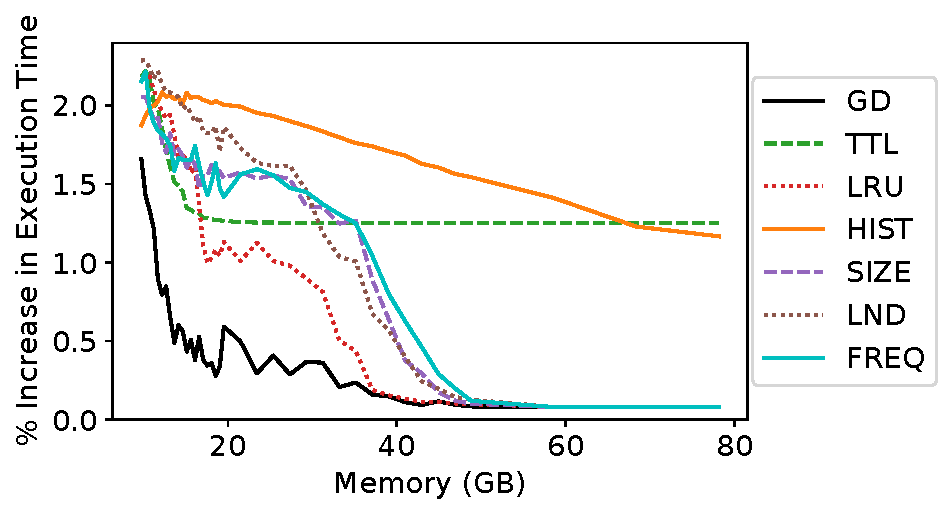
\includegraphics[width=0.37\textwidth]{faascache/faas-keepalive-20/graphs/rep-funcs-392/exec_inc_mem-392-legend.pdf}}
  \hfill 
    \subfloat[Rare functions.     \label{fig:rare-trace-exec}]
{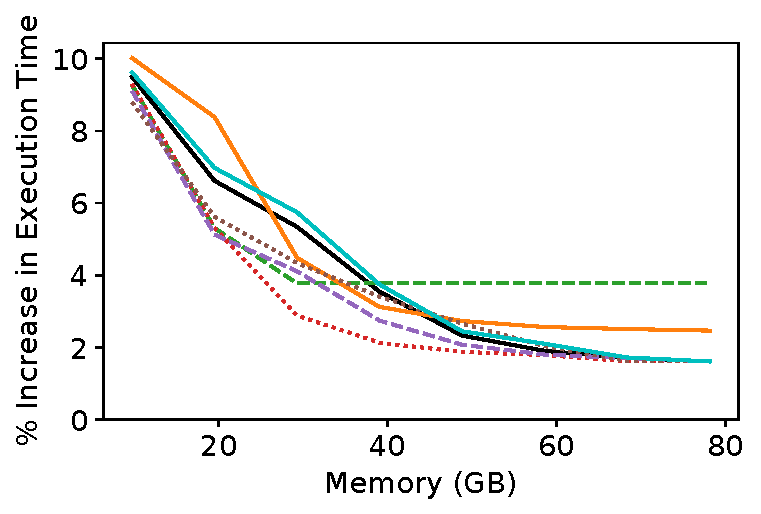
\includegraphics[width=0.3\textwidth]{faascache/faas-keepalive-20/graphs/rare-funcs-1000/exec_inc_mem-1000.pdf}}
\hfill 
  \subfloat[Random sampling.      \label{fig:random-trace-exec}] {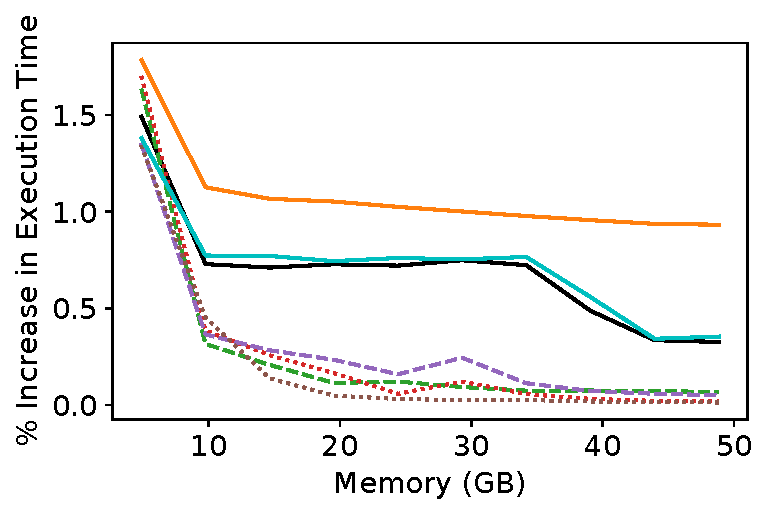
\includegraphics[width=0.3\textwidth]{faascache/faas-keepalive-20/graphs/random-funcs-200/exec_inc_mem-200.pdf}}
\caption{Increase in execution time due to cold starts for different workloads derived from the Azure function trace.}
\label{fig:exec-overheads-all}
\end{figure*}


\begin{figure*}[t]
  \centering
%  \vspace*{\myfigspace}
%  \begin{minipage}[c]{0.7\linewidth}
  \subfloat[Representative functions.\label{fig:rep-trace-cold}] {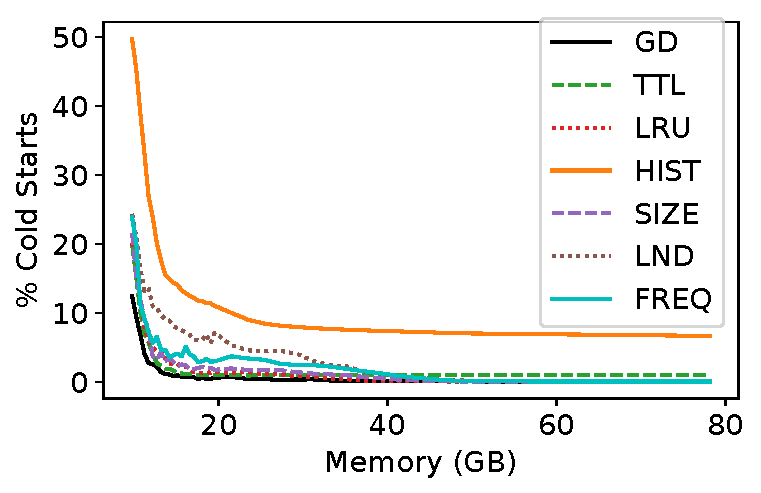
\includegraphics[width=0.33\textwidth]{faascache/faas-keepalive-20/graphs/rep-funcs-392/cold_drop_mem-392-legend.pdf}}
  \hfill
    \subfloat[Rare functions. \label{fig:rare-trace-cold}] {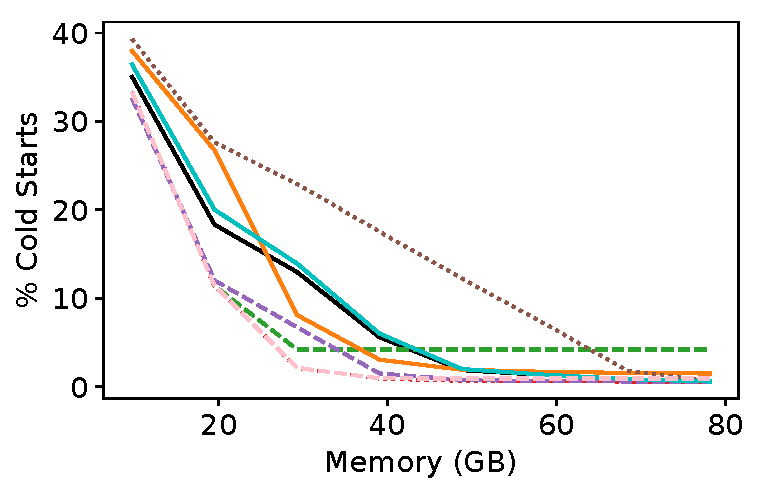
\includegraphics[width=0.33\textwidth]{faascache/faas-keepalive-20/graphs/rare-funcs-1000/cold_drop_mem-1000.pdf}}
  \hfill
  \subfloat[Random sampling. \label{fig:random-trace-cold}]
  {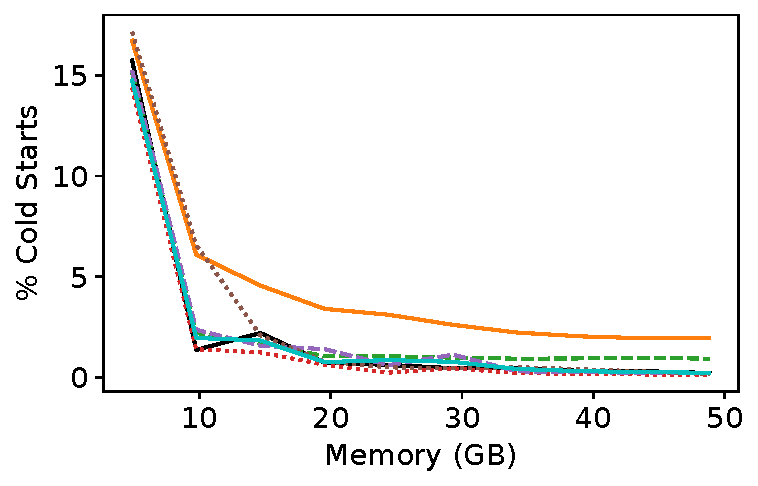
\includegraphics[width=0.33\textwidth]{faascache/faas-keepalive-20/graphs/random-funcs-200/cold_drop_mem-200.pdf}}
    \caption{Fraction of cold starts is lower with caching-based keep-alive. } % for different samples of the Azure function trace.}
      \label{fig:cold starts-all}
%    \end{minipage}
%    \hfill
%    \begin{minipage}[c]{0.29\linewidth}
 %      \begin{figure}
 %     \end{figure}
%    \end{minipage}
\end{figure*}


%%%%%%%%%%%%%%%%%%%%%%%%%%%%%%%%%%%%%%%%%%%%%%%%%%%%%%%%%%%%
\noindent \textbf{Setup, Workloads, and Metrics.}
%
For evaluating different keep-alive performance with different workload types, we use different trace samples from the Azure Function trace~\cite{shahrad_serverless_2020}, which contains execution times, memory sizes, and invocation-timestamps for more than 50,000 unique functions. 
Since our goal is to examine performance at a \emph{server} level, we use smaller samples of this trace for realistic server sizes, and replay them in our discrete-event keep-alive simulator. 
This also allows us to examine the behavior with different \emph{types} of workloads, which is important because our keep-alive policies are designed to be general and workload-agnostic.
We use the following three trace samples (more details in the Table~\ref{tab:trace-deets}): \\
\noindent \textbf{RARE:} A random sample of 1000 of the rarest, most infrequently invoked functions. These functions will usually result in cold starts under a classic 10 minute TTL.  \\
% mention 75% percentile detail?
\noindent \textbf{REPRESENTATIVE:} A sample of 400 functions, sampled from each quartile of the dataset based on frequency---yielding a more representative sample with higher function diversity. \\
\noindent \textbf{RANDOM:} A random sample of 200 functions.

% The FaasCache system is evaluated in Section~\ref{subsec:ow-eval}.
Functions from the FunctionBench~\cite{kim_functionbench_2019} suite are used for generating a realistic workload. 
A single server with 250 GB RAM and 48-core Intel Xeon Platinum 2.10 GHz CPUs is used for running all functions. The server is running modified OpenWhisk (i.e., FaasCache), and Ubuntu 16.04.5. 

\begin{table}
  \centering
  \caption{Size and inter-arrival time (IAT) details for the Azure Function workloads used in our evaluation.}
  \begin{tabular}{lrrr}
    \hline 
    Trace & Num Invocations & Reqs per sec & Avg. IAT \\
    \hline
    Representative & 1,348,162 & 190 /s & 5.4 ms \\
    Rare & 202,121 & 30 /s & 36 ms \\
    Random & 4,291,250 & 600 /s & 1.8 ms \\
    \hline
  \end{tabular}
  \label{tab:trace-deets}
\end{table}



\paragraph{Adapting the Azure Functions Trace.}
The format of the original Azure Function trace~\cite{shahrad_serverless_2020} requires some additional pre-processing and extrapolation for generating a workload.  
The full dataset consists of 14 days of function invocations, and billions of individual invocations. We use the first day's data, and do not consider functions that are never reused (i.e., with less than two invocations). 

The original trace provides memory consumption at the \textit{application} level---with the application made up of multiple functions.
Therefore, we evenly split the memory allocation between all functions in an application.
The dataset provides invocations in minute-wide buckets.
When injecting/replaying the workload, if there is only one invocation in a minute-bucket, it is injected at the beginning of the minute. 
For multiple invocations, they are equally spaced throughout the minute. 

%
The cold start overhead of each function is estimated as {\texttt maximum - average} runtime, and the execution times provided in the dataset are used for this computation. 
The dataset does not account for certain important sources of cold start overheads such as execution environment creation (e.g., Docker).
This unfortunately underestimates the cold start overheads.
However, because it applies uniformly to all functions, it preserves the relative performance of the different keep-alive policies, and does not affect the cache hit ratios. 
%

%These cold start overheads are generally constant, 

%This may not capture all the sources of cold start overhead such as the execution environment creation (e.g., Docker) and 

We are interested in two metrics: the cold start ratio; and the average increase in the execution time due to cold starts.
The increase in execution time is computed by averaging across all function invocations. 

%The latter captures the heterogeneity in function initialization overheads and invocation frequencies. 
%For estimating the time each function spends in explicit initialization, using the workload trace we subtract each functions' average runtime from its maximum runtime. 
%The dataset timings do not include provider overhead, so this initialization time is entirely due to application code.

%%
%Provider cold start overheads can be up to several seconds long, and take up the plurality of a function's execution time.
%Because the dataset does not include provider overhead, it is impossible to assign a realistic number to this cost.
%With these large penalties are not in our simulations, we therefore assume it as 0, but in reality the overhead is roughly constant.
%This causes the global increase in execution time to be smaller than it would be otherwise.
%Including a non-zero cold start cost would apply uniformly across all functions, and thus not change eviction priorities relative to one another.
%The cache hit ratio in Figure~\ref{fig:cold starts-all} would remain unchanged, and the Y-axis (the global increase in execution time) of Figure~\ref{fig:exec-overheads-all} would be scaled up relative to the chosen cold start overhead.
%%

% Using variable, real-world, times would require knowing or randomly assigning the runtime of functions, and would still require stochasticity as provider latency is not constant. 

% Not explaining this in the paper was our biggest “oops”: and there’s a few sources of confusion.
% Here is what we assumed: the dataset doesnt include container startup time, but the included function execution time captures both the function-initialization time (importing packages etc.), and the actual execution.
% So the assumption is that the Max execution time was due to this initialization overhead (which we include in the cold start overhead in our paper).
% The “time functions take to execute after they are ready to run” added to our confusion: we assumed this meant that it is the time when the control is transferred to the FaaS runtime inside the container: which would still incorporate all actual function initialization overheads.
% A contributing factor to making this assumptions was that most OpenWhisk applications do not have a strict explicit initialization, so it is in general not possible to know when a function is truly ready to execute non-idempotent code. 

% And so we end up with pretty small startup overheads, which can be seen from our Figure 5.
% Including container startup time and other overheads would make little difference to relative performance, since the extra overhead would apply to all functions.
% For instance, adding a constant startup penalty for all functions doesnt change their eviction priorities.
% The cache hit ratio (our Figure~\ref{fig:cold starts-all}) would remain unchanged, and the Y-axis of Figure~\ref{fig:exec-overheads-all} would be scaled up depending on the chosen cold start overheads. 

\begin{comment}
Our simulator evaluation uses real-world FaaS usage data from the recently released Azure Function trace~\cite{shahrad_serverless_2020}. 
The entire trace consists of tens of thousands of functions with billions of invocations, making it intractable to simulate the entire dataset.
Trace sampling methodology is important to capture the characteristics of the overall trace, and the scenarios where FaasCache is most effective.
Over half of all functions have an interval arrival time (IAT) over 30 minutes, where IAT is defined as execution time + idle time, guaranteeing them to always have cold starts when using a simple TTL eviction policy.
A tiny 1\% of functions account for nearly 90\% of all invocations, with an IAT of under a minute. 
% Therefore, smaller samples 
Given these extreme disparities, smaller samples must match behaviors of the larger dataset to show their effectiveness.
The full Azure trace can be suitably handled by a cluster of servers, in which case the system behavior is influenced by load-balancing and sharding policies, which our work is orthogonal to.
%Explain the rationale here. 
We generate three day-long traces using the Azure Functions dataset to showcase the effectiveness of FaasCache.
\prat{Insert reuse distance vs. time heatmaps for all these traces in the appendix along with table describing: number of fns, total invocations, avg. inter arrival time, etc.}
\end{comment}

%%%%%%%%%%%%%%%%%%%%%%%%%%%%%%%%%%%%%%%%%%%%%%%%%%%%%%%%%%%%
\subsection{Trace-Driven Keep-Alive Evaluation}

In this subsection, we use the Azure function traces to evaluate different keep-alive policies in our discrete-event simulator. 
% Primary Comparison? Competitors? 
We compare all caching-based variants against the default keep-alive policy in OpenWhisk (10 minute TTL).
% rev 1
When the server is full, this TTL policy evicts containers in an LRU order.
We also evaluate different Greedy-Dual variants: GD is our GDSF policy described in Section~\ref{subsec:gdsf}.
The others are the caching-based variants described in Section~\ref{subsec:variants}: LND is Landlord, and FREQ is LFU. 


%rev 1 
We also compare against the histogram-based keep-alive policy in~\cite{shahrad_serverless_2020}, which is the state of the art technique.
% Section 4.2 of serverless paper 
We have reproduced this policy (HIST) from the details in the paper, and have implemented it in a ``best-effort'' manner without any knowledge of the optimizations in the actual implementation.
This is effectively a ``TTL+Prefetching'' policy: it uses a histogram of \emph{inter-arrival times} to predict future function invocations and eagerly evict warm functions.
It uses timeseries forecasting to capture temporal locality, but does not consider the other function characteristics such as function size and initialization cost. 
The IAT, computed by taking a function's execution time plus the subsequent idle time, between each actual invocation is recorded in minute granularity buckets, tracking up to four hours between executions.
The policy uses ARIMA modeling for those invocations that fall outside this four hour window, we chose not to implement this specific feature due to its complexity, and the fact that it accounted for a minor fraction (\textasciitilde 0.56\%) of all invocations.
From these buckets, a function's coefficient of variation (CoV) is calculated using Welford's online algorithm~\cite{welford}. 
When the function's IAT is predictable (CoV $\leq 2$), the function's historical/customized preload and TTL time are used.
Otherwise, the function has a generic TTL of two hours. 
When an invocation is anticipated, it is brought into memory and kept there until its TTL expires.
A function is evicted when the policy predicts it will not have an invocation in the near future. 
%We chose not to implement the ARIMA modeling for IAT's exceeding four hours for simplicity and the fact it is only applicable to a tiny number of functions.
% \textbf{More details. Histogram size? When created? Online? }


%
The increase in execution time for different traces and for different cache sizes is shown in Figure~\ref{fig:exec-overheads-all}.
% How is this measured?
The increase in execution time is the cold start overheads averaged across all invocations of every function, and captures the user-visible response-time. 
%

For the representative trace (Figure~\ref{fig:rep-trace-exec}), Greedy-Dual reduces the cold start overhead by more than $3\times$ compared to TTL for a wide range of cache sizes (15--80 GB). 
Interestingly, it is able to achieve a low overhead of only 0.5\% at a much smaller cache size of 15GB, compared to other variants, which need 50 GB to achieve similar results---a reduction of cache size by more than $3\times$. 
%
For rare functions (Figure~\ref{fig:rare-trace-exec}), caching-based approaches such as LRU  reduce the cold start overhead by $2\times$ compared to TTL for cache sizes of 40--50 GB. 
This shows that for rare functions, recency is a more pertinent characteristic, and the complex four-way tradeoff used in Greedy-Dual is not necessarily ideal in all workload scenarios. 
For this workload, the HIST policy outperforms TTL, as reported in~\cite{shahrad_serverless_2020}. 
However, it results in 50\% higher cold start overhead compared to caching-based approaches.
Furthermore, because HIST uses only inter-arrival times, it is unable to perform well with heterogeneous representative workloads  (Figure~\ref{fig:rep-trace-exec}). 


Finally, the randomly sampled trace has a large number of infrequent functions because of the low probability of selecting the heavy-hitting functions.
In Figure~\ref{fig:random-trace-exec}, the recency component again dominates, and we see LRU outperforming other variants. 
The equivalence of LRU and TTL-based caching for rare objects has been noted~\cite{basu2017adaptive,jiang2018convergence}, which explains their similar behavior seen in Figure~\ref{fig:random-trace-exec}. 
%closeness of TTL and LRU performance for rare functions in our result. 


\noindent \emph{\textbf{Result:} For representative, diverse workloads, our GD policy can improve the performance and shrink cache sizes by up to $3\times$. For more homogeneous workloads, LRU can outperform current TTL-based approaches by $2\times$.}

%%%
% rev 1 
We can observe from Figure~\ref{fig:exec-overheads-all} that the increase in execution time is generally small ($<10\%$).
This is because of two main factors: the evaluation metric chosen, and the properties of the workload trace. 
The execution time is averaged across \emph{all} function invocations.
However, serverless workloads consist of a large number of very frequently invoked functions. 
The performance of these functions is generally not affected by keep-alive policies, since any policy is going to keep them in the cache because of their high frequency. 
Thus, the difference between non-work-conserving policies such as TTL and Greedy-Dual is masked because of the frequent and popular functions. 
For instance, the average inter-arrival time for all three workloads is less than 36ms, or about 27 function invocations per second. 
Thus, the server is overloaded, and TTL does well even though it is not work-conserving. 
As the IAT grows, the effectiveness of work-conserving caching-based approaches increases compared to TTL, as we shall see in the next subsection. 

%%%%
%While Figure~\ref{fig:exec-overheads-all} focuses on the average increase in execution latency, keep-alive can also reduce the tail latency of functions. Cold start 

%%%%

We see a similar relation and behavior in the miss-ratio curves shown in Figure~\ref{fig:cold starts-all}. 
Due to function heterogeneity, the cold start overheads are not strictly correlated with cache miss ratios, and thus the differences between policies is different compared to the previously described actual cold start overheads. 
% \prat{Write after colors are fixed.}
Classic miss-ratio curves do not consider the miss \emph{cost} (i.e., initialization cost), which is an important metric that is optimized by the Greedy-Dual approach.
Thus, in general, even in object caching contexts, miss-ratio curves deviate from the actual performance---a behavior that we also observe. 

%%%%%%%%%%%%%%%%%%%%%%%%%%%%%%%%%%%%%%%%%%%%%%%%%%%%%%%%%%%%
\subsection{OpenWhisk Evaluation}
\label{subsec:ow-eval}



\begin{figure}
  \centering
  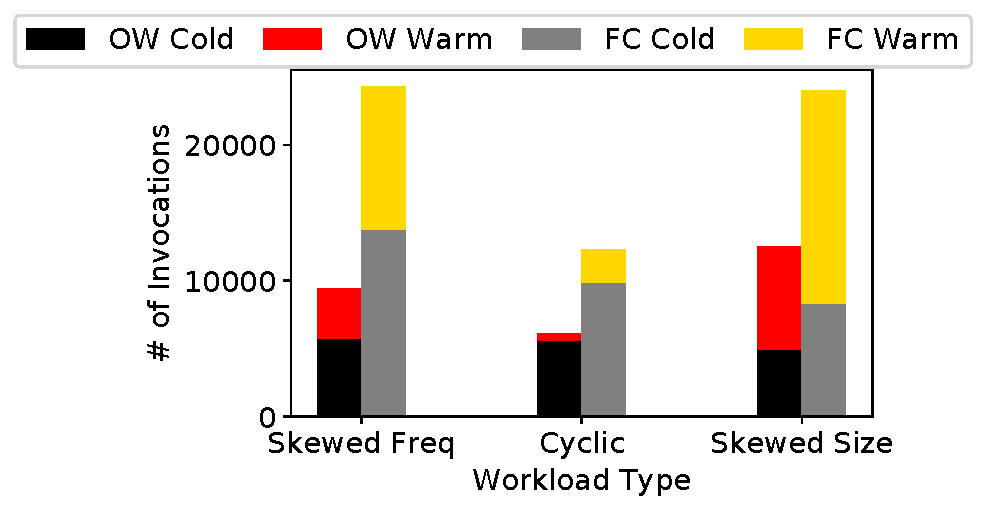
\includegraphics[width=0.6\textwidth]{faascache/faas-keepalive-20/graphs/litmus_tests/litmus_2_stacked.pdf}
  \caption{FaasCache runs 50 to 100\% more cold and warm functions, for skewed workload traces.}
  \label{fig:litmus_2}  
\end{figure}


In this subsection, we evaluate the performance of the FaasCache system on real functions. 
We focus on the performance of FaasCache's Greedy-Dual keep-alive implementation, and compare it to the vanilla OpenWhisk system which uses a 10 minute TTL.


% rev1 1
In contrast to the previous subsection in which we showed the average performance for different cache sizes, we will now also focus on the inverse problem: for a fixed server size, how much more load can be handled with FaasCache? 
By leveraging Greedy-Dual caching, FaasCache is able to reduce cold starts. 
This also reduces the number of \emph{dropped} requests. %

OpenWhisk buffers and eventually drops requests if it cannot fulfill them.
Because FaasCache more effectively selects evictions, its higher hit rate results in functions finishing faster, allowing more functions to be executed in the same time frame.  
%
\begin{table}
  \centering
  \caption{FaaS workloads are highly diverse in their resource requirements and running times. The initialization time can be significant and is the cause of the cold start overheads, and depends on the size of code and data dependencies.}
  \begin{tabular}{lrrr}
    \hline 
    Application & Mem size & Run time & Init. time \\
    \hline
    ML Inference (CNN) & 512 MB & 6.5 s & 4.5 s \\
    Video Encoding & 500 MB & 56 s & 3 s \\
    Matrix Multiply & 256 MB & 2.5 s & 2.2 s \\
    Disk-bench (\texttt{dd})  & 256 MB & 2.2 s & 1.8 s \\
    Image Manip & 300 MB & 9 s & 6 s \\
    Web-serving & 64 MB & 2.4 s & 2 s \\
    Floating Point & 128 MB & 2 s & 1.7 s \\
    \hline
  \end{tabular}
  % \vspace*{\myfigspace}
  \label{tab:fc:workloads}
  %\vspace*{\myfigspace}
\end{table}

To examine the effect of Greedy-Dual keep-alive on cold start and dropped requests, we use a workload trace comprising of four different functions: Disk-bench, ML inference, Web-serving, and Floating-point, described in Table~\ref{tab:fc:workloads}.

In Figure~\ref{fig:litmus_2}, we use different kinds of \emph{skewed} workloads: with a single function having a different frequency, a cyclic access pattern, and a skewed workload with 2 sizes. 
We see that FaasCache's keep-alive can increase the number of warm invocations by between 50 to 100\% compared to OpenWhisk's TTL.
The difference in the total number of requests served (warm+cold) is because OpenWhisk drops a significant number of requests due to its high cold start overhead and resultant system load. 
%
Thus with FaasCache, the total number of requests that are served also increases by $2\times$. 

%rev 1 above 
%Interestingly, OpenWhisk drops a significant number of requests, which is the cause of the different total served requests. 
%

% The impact on the different function performances can be seen in Figure~\ref{fig:faasbench}.
% For this figure, to generate the workload, the first three functions have an inter-arrival time of 1500 ms, and the fourth (floating-point) has a lower IAT of 400 ms. 

%a disk-based one, web-page serving, floating-point trigonomotry operations in numpy, and a convolutional neural network inference (TensorFlow with which model?). % A detailed description of these workloads is required.

% Explain what is the iat distribution and (other details? ).


% 32 GB wted_increase vanilla 11.964% cache 11.528%
% 48 GB wted_increase vanilla 6.184% cache 0.624%


\begin{figure}[t]
  \centering
\includegraphics[width=0.6\textwidth]{faascache/faas-keepalive-20/graphs/litmus_tests/faasbench_48_cold_hot-legend.pdf}
\caption{FaasCache increases warm-starts by more than $2\times$, which also reduces system load and dropped functions.}
\label{fig:faasbench}
\end{figure}


\begin{comment}
\begin{figure}[t]
  \centering
\subfloat[48 GB   \label{fig:faasbench-stacked-48}]
{ \includegraphics[width=0.3\textwidth]{../graphs/litmus_tests/faasbench_48_cold_hot-legend.pdf}}
\hfill 
  \subfloat[32 GB   \label{fig:faasbench-stacked-32}]
{  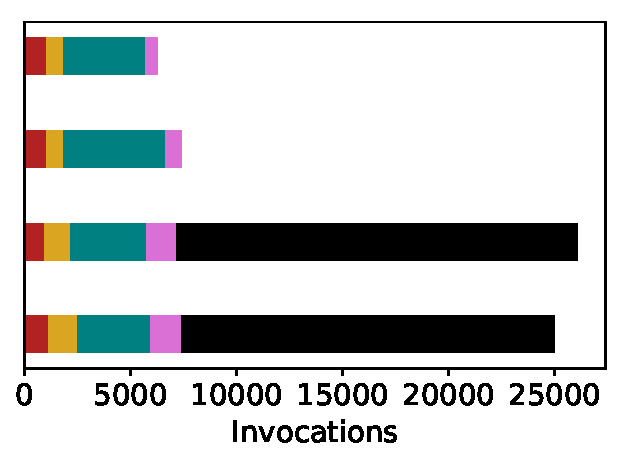
\includegraphics[width=0.17\textwidth]{../graphs/litmus_tests/faasbench_32_cold_hot.pdf}}
\caption{Impact of keep-alive on different function types.}
\label{fig:faasbench}
\end{figure}
\end{comment}

% Figure~\ref{fig:faasbench-stacked-32} shows the number of cold and dropped requests for the different functions, with a medium cache size of 32 GB.
% This setup is intended to evaluate our system in resource constrained environments.
% We see that dropped requests dominate, and FaasCache's more effective keep-alive serves 45\% of requests, while OpenWhisk only serving ~40\%.
% At the same time, warm starts improve 17\% using FaasCache.


Next, we use the skewed frequency workload and use functions from Table~\ref{tab:fc:workloads} to evaluate the impact on real applications. 
%The impact on the different function performances can be seen in Figure~\ref{fig:faasbench}.
To generate the workload, the CNN, DD, and Web-serving functions have an inter-arrival time of 1500 ms, and the Floating-point function has a lower IAT of 400 ms. 
%
Figure~\ref{fig:faasbench} shows the breakdown of different function invocations for this workload on a 48 GB server.
Interestingly, OpenWhisk drops a significant number (50\%) of requests due to the its high cold start overheads.
FaasCache increases the warm requests by more than $2\times$. 
Interestingly, the \emph{distribution} of warm starts is also different. 
FaasCache's Greedy-Dual policy prioritizes functions with higher initialization times, but penalizes those with large memory footprints. 
Because the floating-point function has a high initialization overhead (Table~\ref{tab:fc:workloads}), it sees a $3\times$ increase in hit-ratio compared to OpenWhisk.
\emph{In practical terms, the improvement in keep-alive results in a $6\times$ reduction in the application latency.
}
%The ML inference function has an 8\% lower warm hit rate than the other functions, as it gets de-prioritized because of it's high memory needs.


%When the cache size is increased to 48 GB (Figure~\ref{fig:faasbench-stacked-48}), FaasCache doesn't drop a single request, while OpenWhisk still can't serve 50\% of them.
%For the same workload, Figure~\ref{fig:faasbench-stacked-32} shows the distribution of cold and warm starts for a larger cache size of 32 GB.
%The number of warm starts increases by nearly 20\% compared to OpenWhisk.
% FaasCache's Greedy-Dual policy prioritizes functions with higher initialization times, the CNN function sees a 53\% higher warm starts, wheres Z function only sees X\% increase compared to OpenWhisk. 
% The floating point function has a very high initialization overhead (1.7 of the total 2 seconds), and thus sees its warm-start rate increase the most, by 40\%. 

\begin{comment}
At a smaller cache size of 32 GB shown in Figure~\ref{fig:faasbench-stacked-32}, the number of dropped requests dominate.
This setup is intended to evaluate our system in resource constrained environments.
FaasCache's more effective keep-alive serves 45\% of requests, while OpenWhisk drops nearly 60\%.
Warm-starts increase by 17\% with FaasCache. 
\end{comment}

\noindent \emph{\textbf{Result:} FaasCache can increase the number of warm-starts by $2\times$ to $3\times$ depending on the function initialization overheads and workload skew. This results in lower system load, which increases the number of requests FaasCache can serve by $2\times$.}

%\prat{CPU Graph not required, but just the average numbers will do.}

%%%%%%%%%%%%%%%%%%%%%%%%%%%%%%%%%%%%%%%%%%%%%%%%%%%%%%%%%%%%
\subsection{Effectiveness of Provisioning Policies}
All our previous results have been with a statically allocated server, and 
we now illustrate the effectiveness of our dynamic vertical scaling policy described in Section~\ref{subsec:dynamic}.
The goal is to dynamically adjust the cache size based on the workload. 
Our  policy seeks to keep the miss speed (cold starts per second) close to a pre-specified target. 
This is shown in Figure~\ref{fig:dynamic}---the target is 0.0015 misses per second. 
In this experiment, the cache resizing is done only when the miss speed error exceeds 30\%, and we can see that the cache size increases with the miss speed, and decreases with it. 
Without the dynamic scaling, a conservative provisioning policy would result in a constant, 10,000 MB size. 
In contrast, the average cache size with our proportional controller is less than 7,000 MB.
This 30\% reduction means that FaaS providers can reduce their provisioned resources without compromising on performance.
The freed-up resources can be used to accommodate additional cloud workloads (such as co-located VMs and containers). 
Our dynamic scaling is extremely conservative: increasing its agressiveness by reducing the error tolerance below 30\% will reduce  average server size,
%but cause a larger number of small memory-size  changes, which we wish to avoid.
but we seek to avoid the resultant small changes to memory-size to minimize fragmentation. 
%avoid why?? 

\begin{figure}[t]
  \centering 
  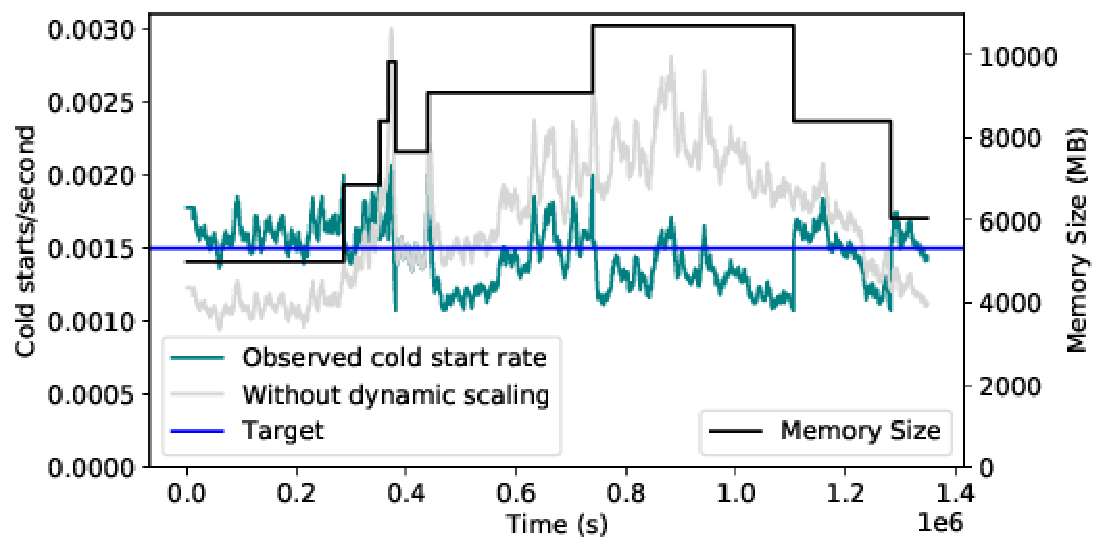
\includegraphics[width=0.6\textwidth]{faascache/faas-keepalive-20/graphs/dyn-scale-392-b.pdf}
  \caption{With dynamic cache size adjustment, the cold starts per second are kept close to the target (horizontal line), which reduces the average server size by 30\%. }
  \label{fig:dynamic}
\end{figure}

%%% Local Variables:
%%% mode: latex
%%% TeX-master: "paper"
%%% End:


\section{Related Work}
\label{sec:related}

\noindent \textbf{Locality} is an important design and optimization principle in FaaS---and is a fundamental result of code and data initialization required for each function.
Keep-alive policies for warm-starts apply temporal locality~\cite{roy2022icebreaker, ebrahimi2024cold, vahidinia2022mitigating, shahrad2020serverless} and caching~\cite{faascache-asplos21, sundarrajan2017footprint} principles for the CPU memory pool; load balancing also benefits from stickiness~\cite{package-cristina-19, faaslb-hpdc22, abdi2023palette}.
Our work extends these principles to GPU functions via locality enhanced fair queuing and proactive memory management. 

% Bursty functions can cause load imbalance and queuing on systems, and intelligent queuing can avoid additional latency~\cite{yan2020hermes}.

\noindent \textbf{GPUs in serverless computing} is already a rich and fast-growing area of research. 
A big portion of prior work~\cite{naranjo2020accelerated, fingler2022dgsf, kim_gpu_2018} focuses on disaggregated accelerators, with GPUs accessed over the network using techniques such as rCUDA~\cite{duato2010rcuda}.
In contrast, we look at local GPUs without remote execution. 
Using FaaS-inspired abstractions to provide GPU acceleration as a service is also common: applications are broken down into kernels which can be run ``anywhere''.
Kernel-as-a-Service~\cite{pemberton2022kernel} and Molecule~\cite{du2022serverless} are two examples of this approach, where the main challenges are designing and providing efficient and usable API-remoting mechanisms. 
\cite{juan_reducing_2023} also uses remote memory pooling to address the exacerbated cold-start problems for GPUs, and also proposes parallel data-dependency and compute context prefetching through code-level optimizations. 
Paella~\cite{ng2023paella} similarly breaks apart model inference tasks into CUDA kernel launches to minimize scheduling ``bubbles''.
These and other recent~\cite{sage_zhao_towards_2024} specialized code-modifying techniques are orthogonal to our work, since we require general black-box functions.

% MIG Over-allocation causes fragmentation, and the opposite approach will reduce performance or prevent function execution due to insufficient resources.
% Assigned partitions can lead to underutilization due to fragmentation from poor placement and function idle periods. Idle functions cause immediate underutilization, which could be alleviated via temporal sharing complicating fixed hardware partition management even further.

The popularity of \textbf{ML inference} has resulted in a large number of specialized solutions to efficient GPU scheduling, which have similar challenges, but a different optimization spaces: inference resource requirements are much more deterministic~\cite{gujarati2020serving} and thus amenable to data-driven optimization~\cite{ali2022optimizing}, and the lack of isolation among requests provides many locality-enhancing and batching opportunities~\cite{yang2022infless, satzke2020efficient}. 
For instance, both FaST-GShare~\cite{gu2023fast} and TGS~\cite{tgs_wu2023transparent} leverage profiles of ML workloads to monitor GPU utilization and use 2d bin-packing (with time and memory dimensions) to schedule inference workloads.

%Both of these automatically move memory off of the device when kernels are done, and don't have to worry about applications holding onto device memory when idle.

%  profiles ML workloads to monitor how much of the GPU it utilizes, then uses this information to schedule inference tasks on GPUs to maximize utilization.
% ML inference tasks have fixed sized memory and kernel usages (known tensor sizes, etc.) and this is an effective approach.
% Other applications can have arbitrary and changing requirements, especially when one considers that function arguments are the main determiner of resource usage, so this idea breaks down when shifting to black-box applications.

Finally, \textbf{scheduling} is crucial for FaaS performance, with key tradeoffs in late vs. early binding~\cite{kaffes2021practical, kaffes_hermod_2022}.
Efficiency and fairness tradeoffs in GPU scheduling have been recently resolved~\cite{mo_optimal_2024}, but only in the offline context with a limited number of batch jobs with known utilities. 

%%% Local Variables:
%%% mode: latex
%%% TeX-master: "paper"
%%% End:


\section{Conclusion}
%\vspace*{\subsecspace}

The main insight in this paper is the isomorphism between function keep-alive and object caching.
Using it, sophisticated caching policies can be applied to FaaS.
Our Greedy-Dual based keep-alive policy can reduce cold-start overheads by up to $4\times$ compared to simple policies.
The caching analogy can also be used to enhance resource provisioning. 


% use section* for acknowledgment
\ifCLASSOPTIONcompsoc
  % The Computer Society usually uses the plural form
  \section*{Acknowledgments}
\else
  % regular IEEE prefers the singular form
  \section*{Acknowledgment}
\fi
The authors would like to thank Jose Viteri and Robinson Flores from ESPOL, who helped analyze the Azure trace data with respect to burstiness and workload characterization of high- versus low-priority functions (Figure~\ref{fig:bursty:allworkloads} and Section~\ref{sec:motivation:workload}).
% This work was funded by NSF OAC-ICICLE 


{
\bibliographystyle{acm}
\interlinepenalty=10000 %%%%For fixing url-related errors only 
\bibliography{faas,faas-asplos,lb,differentiated}
%\bibliography{bagsjobs}
}



%\vspace{-15pt}
\begin{IEEEbiography}[{\includegraphics[width=1in,height=1.25in,clip,keepaspectratio]{bios/INSERTHERE.jpg}}]
{Alexander Fuerst} is a Ph.D. candidate in the Department of Intelligent Systems Engineering at Indiana University Bloomington. He received a BS in Computer Engineering from Indiana University Bloomington in 2019.  His research interests lie primarily in \end{IEEEbiography}


\begin{IEEEbiography}[{\includegraphics[width=1in,height=1.25in,clip,keepaspectratio]{bios/prateeks.jpg}}]{Prateek Sharma}
  is an an assistant professor of Intelligent Systems Engineering at Indiana University in Bloomington. He has a PhD in Computer Science from  
the University of Massachusetts Amherst. His current research
  focuses on Cloud Computing, Operating Systems, and
  Virtualization. Sharma received his masters degree in Computer Science from
  Indian Institute of Technology, Bombay. Contact him at
  prateeks@iu.edu.
\end{IEEEbiography}


\begin{IEEEbiography}[{\includegraphics[width=1in,height=1.25in,clip,keepaspectratio]{bios/cabad_headshot.JPG}}]{Cristina L. Abad} received the MS and PhD degrees in CS from the University of Illinois at Urbana-Champaign. She is currently an associate professor at Escuela Superior Politecnica del Litoral, ESPOL, in Ecuador, where she leads the Distributed Systems Research Lab (DiSEL). Her research interests include intersection of distributed systems and performance engineering. Contact her at cabad@fiec.espol.edu.ec.
\end{IEEEbiography}


\end{document}

%%% Local Variables:
%%% mode: latex
%%% TeX-master: t
%%% End:
